%% Type de document et encodage de la police
\documentclass[a4paper]{article}
\usepackage[utf8x]{inputenc}
\usepackage[T1]{fontenc}
\usepackage[colorlinks=true, allcolors=black]{hyperref}
% \usepackage[french]{babel}

%% Initialise la taille des pages et des marges
\usepackage[a4paper, top=3cm, bottom=3cm, left=2cm, right=2cm, marginparwidth=2cm]{geometry}

%% Packs utiles
\usepackage{amsmath}
\usepackage{graphicx}

%% Commandes perso
\renewcommand{\arraystretch}{1.2} %% row 20% longer
\renewcommand{\contentsname}{Table des matières}

%% Pour les exemples
\usepackage{mdframed}
\newmdenv[topline=false, bottomline=false, rightline=false, skipabove=\topsep, skipbelow=\topsep]{example}

%% Pour les diagrammes
\usepackage{tikz}
\tikzstyle{incolore} = [rectangle, rounded corners, draw=black, minimum height=1cm, minimum width=3cm, text width=3cm, text centered]


\title{Notes OS Open Source Pratique}
\author{Grégoire Roumache}
\date{Octobre 2020}

\begin{document}

\maketitle

\tableofcontents

\begin{center} \rule{0.95\linewidth}{0.1mm} \end{center}















\section{Voir les logs}




\textbf{Attention !} Quand on a un problème, vérifier les logs.
\begin{itemize}
    \item \textcolor{red}{\textbf{Meilleure option}} : \texttt{journalctl -xe}
    \item Voir les logs en continu : \texttt{journalctl -fxe}
    \item Voir le statut d'un service : \texttt{systemctl status <service>}
    \item Voir les derniers logs : \texttt{dmesg | less}
    \item Lister les fichiers logs : \texttt{ls /var/log}
    \item Voir les derniers logs système (sauf auth) : \texttt{tail [-n <nb\_lignes>] /var/log/syslog}
    \item Voir les logs en continu : \texttt{tail -f /var/log/syslog}
\end{itemize}
\textbf{Logs Apache2}:
\begin{itemize}
    \item Les logs sont dans le dossier : \texttt{/var/log/apache2/}
    \item En cas de problème pour relancer apache : \texttt{tail /var/log/apache2/error.log}
\end{itemize}
Commandes cool pour lister les services (ceux qui ont un problème sont en rouge) :
\begin{itemize}
    \item \texttt{systemctl list-units -{}-type service -all}
    \item \texttt{systemctl list-unit-files -{}-type service}
\end{itemize}
Pour déboguer une configuration dns :
\begin{itemize}
    \item \texttt{sudo named-checkconf -z}
\end{itemize}















\section{Touver un fichier}





\texttt{find <folder> -name <nom\_fichier>}




















\section{Révisions}










\subsection{Manipulation sur l'installation}





\begin{itemize}

\item Lancer l'installation en mode texte en ANGLAIS dans une VM virtualbox avec un DD de taille dynamique de 20 Go.

\item Suivre les instructions en configurant correctement le clavier (belge), etc.

\item Réaliser manuellement le partitionnement suivant :
\begin{itemize}
    \item sda1 : /boot = 256 Mo
    \item sda2 : swap = 1 Go
    \item sda3 : / = 10 Go
    \item sda4 : partition logique
    \begin{itemize}
        \item sda5 : /home = 2 Go
        \item sda6 : /tmp = 2 Go
        \item free space = max
    \end{itemize}
\end{itemize}

\item Compte utilisateur : user. Mots de passe : tttttt.

\item Choisir comme mot de passe pour root : tttttt.

\item N'installer que le système de base.

\begin{example}
    Guide pour l'installation:
    \begin{enumerate}
        \item lancer l'installation \textit{sans} le mode graphique
        \item prendre langue: \textit{english}, pays: \textit{other -> europe -> Belgium}
        \item prendre pays des paramètres par défaut: \textit{united states}, clavier: \textit{belgian}
        \item hostname: \textit{debian}, laisser vide le domain name
        \item mot de passe root: \textit{tttttt} (= $ 6 \times t $), utilisateur: \textit{user}, mot de passe user: \textit{tttttt}
        \item lancer le partitionnement en mode manuel
        \item sur \textit{SCI1 (0,0,0) (sda) ...}, taper \textit{enter}, puis sur \textit{yes}
        \item sur \textit{free space}, taper \textit{enter}, puis \textit{create a new partition}
        \begin{enumerate}
            \item 256 MB - primary - beginning - ext4 – /boot – bootable flag = \textit{on}
            \item 1 GB - primary - beginning - swap area
            \item 10 GB - primary - beginning - ext4 - /
            \item 2 GB - logical - beginning - ext4 - /home
            \item 2 GB - logical - beginning - ext4 - /tmp
        \end{enumerate}
        \item taper \textit{enter} sur \textit{finish partitionning and write changes to disk}
        \item dans \textit{software selection}, ne sélectionner que \textit{standard system utilities}
        \item installer GRUB
    \end{enumerate}
\end{example}

\item Si besoin, ajouter un proxy. Dans quelle situation cela peut-il être utile ?
\begin{example}
    En général, un proxy est utilisé pour:
    \begin{itemize}
        \item accélérer la navigation
        \item la sécurité du réseau local
        \item le filtrage et l'anonymat
    \end{itemize}
\end{example}

\item Prendre le miroir réseau par défaut.

\item Installer le boot manager dans le MBR. Où peut-il être encore installé ? Expliquer la différence et comment cela fonctionne.
\begin{example}
    \begin{itemize}
        \item MBR = master boot record = 1er secteur d'un disque dur
        \item On peut aussi l'installer sur n'importe quelle partition àpd moment où il y a un flag \texttt{boot} (seulement UEFI, pas BIOS).
        \item La différence est que avec le MBR, on charge le GRUB directement. Avec l'autre méthode, l'UEFI va chercher la partition avec le boot dans la table de partitions.
    \end{itemize}
\end{example}

\item Quel est le boot manager installé ?
\begin{example}
    GRUB = grand unified bootloader
\end{example}

\item Finir l'installation, se connecter au système, vérifier que tout fonctionne correctement.
\begin{example}
    \begin{enumerate}
        \item Pour avoir accès aux commandes système telles que: \texttt{useradd}, \texttt{mkfs} ou \texttt{fdisk}:
        \begin{itemize}
            \item \texttt{export PATH="\$PATH:/sbin"}
        \end{itemize}
        \item Ajouter \texttt{user} au sudoers:
        \begin{itemize}
            \item \texttt{su root}
            \item \texttt{apt install sudo}
            \item \texttt{usermod -aG sudo user}
            \item \texttt{exit}
        \end{itemize}
    \end{enumerate}
\end{example}

\end{itemize}










\subsection{Rappel sur la configuration réseau}





\begin{itemize}

\item Vérifier la configuration IP : \texttt{ip addr show}

\item Vérifier la MAC address : \texttt{ip link show <interface>}.

\item Vérifier la default gateway : \texttt{ip route list}.

\item Vérifier les serveurs DNS \texttt{cat /etc/resolv.conf} (ou \texttt{systemd-resolve –status}).

\item Adresse IP statique:
\begin{itemize}
    \item Nettoyer : \texttt{ip addr flush dev enp0s3}
    \item Ajouter : \texttt{ip addr add 192.168.50.5/24 dev enp0s3}
    \item Supprimer : \texttt{ip addr del 192.168.50.5/24 dev enp0s3}
\end{itemize}

\item Adresse IP dynamique :
\begin{itemize}
    \item \texttt{dhclient [-v ] enp0s3}
    \item \texttt{pkill dhclient}
\end{itemize}

\item Adresses IP supplémentaires : \texttt{ip addr add 192.168.50.50/24 dev enp0s3}

\item Nom d’hôte : \texttt{hostname [nouveauNom]}

\item Passerelle par défaut \& Passerelles supplémentaires :
\begin{itemize}
    \item \texttt{ip route add 10.10.20.0/24 via 192.168.50.100}
    \item \texttt{ip route del 10.10.20.0/24}
    \item \texttt{ip route add default via 192.168.50.100}
    \item \texttt{ip route del default}
\end{itemize}

\item Mac Address : \texttt{ip link set dev interface address XX:XX:XX:XX:XX:XX}

\item Carte réseau :
\begin{itemize}
    \item \texttt{ip link set enp0s3 up}
    \item \texttt{ip link set enp0s3 down}
\end{itemize}

\item Déconfigurer - arrêter / Configurer-activer le réseau une carte :
\begin{itemize}
    \item \texttt{ifup enp0s3}
    \item \texttt{ifdown enp0s3}
\end{itemize}

\item Paramètres de base (relancer le service réseau : \texttt{systemctl restart networking}) :
\begin{verbatim}
auto enp0s3
iface enp0s3 inet static
address X.X.X.X
netmask X.X.X.X
gateway X.X.X.X
dns-nameservers X.X.X.X Y.Y.Y.Y
\end{verbatim}

\item Mac Address : fichier \textit{/etc/network/interfaces} : \texttt{hwaddress ether 00:01:04:1b:2C:1F}

\end{itemize}










\subsection{Rappels sur la gestion des utilisateurs et des fichiers}





\begin{itemize}

\item Se connecter en tant qu'utilisateur dans une console : \texttt{su user}.

\item Devenir root temporairement : \texttt{su root}.

\item Lister à l'écran les fichiers /etc/passwd et /etc/group : \texttt{cat <fichier>}.

\item Expliquer la signification des champs pour l’utilisateur root, user, et le groupe user: \texttt{man 5 passwd}.

\item Créer les groupes grp1, grp2, et grp3. Le GID du groupe 3 doit être 999 : \texttt{groupadd [-g <gid>] <groupe>}.

\item Créer les utilisateurs user1, user2 et user3 qui doivent avoir respectivement comme groupe principal grp1, grp2, et grp3 :
\begin{example}
    \begin{itemize}
        \item \texttt{adduser [-{}-ingroup <group>] <user>}
        \item vérification : \texttt{groups <user>}
    \end{itemize}
\end{example}

\item user2 doit pouvoir accéder aux fichiers des groupes grp2 et grp3, avec les mêmes droits que ces derniers. Vérifier que c'est bien le cas.

\item Supprime le groupe 3. Est-ce possible ? Pq ? --- Non car grp3 est le groupe primaire de user3.

\item Supprime l'utilisateur 3 en gardant sans supprimer le répertoire personnel ni le groupe 3.

\item À qui appartient le répertoire /home/user3 désormais ? Pq ? \texttt{stat /home/user3}, UID = 1003/unknown.

\item Comment retrouver les fichiers qui appartenaient à l'utilisateur 3 ou au groupe 3 ? Comment les supprimer ?
\begin{example}
    \begin{itemize}
        \item \texttt{find <dossier> -group <group>}
        \item \texttt{find <dossier> -gid <user-gid>}
        \item \texttt{find <dossier> -group <group> | xargs rmdir}
        \item \texttt{find <dossier> -gid <user-gid> | xargs rmdir}
        \item (\texttt{sudo find <dossier> -gid <user-gid> | xargs sudo rmdir})
    \end{itemize}
\end{example}

\item Se connecter dans une autre console virtuelle (non graphique !) avec root
\begin{example}
    \begin{itemize}
        \item appuyer sur : \texttt{ctrl+alt+f2}
        \item il y a des consoles de \texttt{f1} à \texttt{f6}
    \end{itemize}
\end{example}

\item Modifier les mots de passe des utilisateurs créés précédemment : \texttt{sudo passwd <user>}.

\item Qui d'autre que root peut modifier un mot de passe ? L'utilisateur lui-même.

\item Comment user2 peut-il devenir temporairement user1 ? Comment prendre complètement l'environnement de user1 ? \texttt{su user1}

\item Se déconnecter des différentes consoles : \texttt{exit}.

\item Désactiver les comptes user1 et user2 via 2 méthodes différentes et vérifier.
\begin{example}
    Méthode 1:
    \begin{itemize}
        \item \texttt{usermod -{}-lock -{}-expiredate 1970-01-02 <username>}
    \end{itemize}
    Méthode 2:
    \begin{itemize}
        \item \texttt{chage -E 0 username}
    \end{itemize}
\end{example}

\item Réactiver les comptes.
\begin{example}
    Méthode 1:
    \begin{itemize}
        \item \texttt{usermod -{}-unlock -{}-expiredate '' <username>}
    \end{itemize}
    Méthode 2:
    \begin{itemize}
        \item \texttt{chage -E -1 username}
    \end{itemize}
\end{example}

\item Créer un nouveau répertoire rep2 contenant un fichier vide fic2 dans /tmp et regarder les droits associés à ces nouveaux fichiers.
\begin{example}
    \begin{itemize}
        \item \texttt{mkdir /tmp/rep2}
        \item \texttt{touch /tmp/rep2/fic2}
        \item \texttt{namei -mo /tmp/rep2/fic2}
    \end{itemize}
    \texttt{drwxr-xr-x} ($ \implies $ \texttt{d rwx r-x r-x})
    \begin{itemize}
        \item \texttt{d} : c'est un répertoire.
        \item \texttt{rwx} : le propriétaire peut lire, écrire et exécuter.
        \item \texttt{r-x} : le groupe peut lire et exécuter le fichier, pas le modifier.
        \item \texttt{r-x} : le reste peut lire et exécuter le fichier, pas le modifier.
    \end{itemize}
\end{example}

\item Changer les droits du fichier fic2 afin que personne ne puisse les modifier.
\begin{example}
    \begin{itemize}
        \item À qui s'applique le changement:
        \begin{itemize}
            \item u : user = utilisateur
            \item g : group = groupe
            \item o : others = autres
            \item a : all = tous
        \end{itemize}
        \item La modification que l'on veut faire:
        \begin{itemize}
            \item + : ajouter
            \item - : supprimer
            \item = : affectation
        \end{itemize}
        \item Le droit que l'on veut modifier:
        \begin{itemize}
            \item r : read = lecture
            \item w : write = écriture
            \item x : execute = exécution
        \end{itemize}
    \end{itemize}
    \texttt{chmod a-w /etc/rep2/fic2}
\end{example}

\item Essayer de supprimer le fichier /tmp/rep2/fic2. Est-ce possible ? Pourquoi ?
\begin{example}
    \begin{itemize}
        \item \texttt{rm /tmp/rep2/fic2}
    \end{itemize}
    Ça marche. Je suppose que c'est parce que je suis le propriétaire.
\end{example}

\item Changez le propriétaire de rep2 et fic2 à user2 et le groupe propriétaire à grp3. Essayer de supprimer le fichier avec user2
\begin{example}
    \begin{itemize}
        \item changer le propriétaire (change owner) : \texttt{sudo chown <user> <fichier>}
        \item changer le groupe (change group) : \texttt{sudo chgrp <group> <fichier>}
    \end{itemize}
\end{example}

\item Modifier le umask. Est-ce d'application pour les comptes pré existants ? (si non que faire?). Et pour les futurs comptes crées ?
\begin{example}
    \begin{itemize}
        \item afficher l'umask : \texttt{umask -S}
        \item changer l'umask : \texttt{umask u=rwx,,g=rx,o=rx}
    \end{itemize}
\end{example}

\item Modifier les droits par défaut à 0700 pour les futurs fichiers des utilisateurs, mais aussi ceux déjà présents : \texttt{umask 0700}.

\item Créez un lien symbolique dans votre répertoire personnel pointant sur /var/log : \texttt{ln -s <fichier> <lien>}.

\item Créez un lien symbolique dans votre répertoire personnel pointant sur un fichier texte : \texttt{ln -s <fichier> <lien>}.

\item Créez un lien physique dans votre répertoire personnel pointant sur le dossier /tmp/votreNom : \texttt{ln <fichier> <lien>}.

\end{itemize}















\section{Administration de base}





\begin{itemize}

\item Installer le logiciel ethtool : \texttt{sudo apt install ethtool}.

\item Ajouter les paquets contrib et non-free.
\begin{example}
    \begin{itemize}
        \item \texttt{sudo nano /etc/apt/sources.list}
        \begin{verbatim}
    # ajouter : contrib non-free, à la fin des lignes avec des urls
    deb http://http.deb.debian.org/debian stable main contrib non-free
        \end{verbatim}
        \item \texttt{sudo apt update}
    \end{itemize}
\end{example}

\item Récupérer les informations sur ce paquet : \texttt{sudo apt show ethtool}.

\item Désinstaller ce paquet complètement : \texttt{sudo apt remove ethtool}.

\item Mettre à jour votre distribution : \texttt{sudo apt full-upgrade}.

\end{itemize}










\subsection{Manipulation - DPKG}





\begin{itemize}

\item Téléchargez et Installez le paquet iptraf
\begin{example}
    \begin{itemize}
        \item chercher le fichier sur le serveur ftp : \texttt{http://ftp.de.debian.org/debian/pool/}
        \item \texttt{wget http://ftp.de.debian.org/debian/pool/main/i/iptraf/iptraf\_3.0.0-8.1\_amd64.deb}
        \item \texttt{dpkg -i iptraf\_3.0.0-8.1\_amd64.deb} (ou : \texttt{ls | grep iptraf | xargs sudo dpkg -i})
    \end{itemize}
\end{example}

\item Vérifier si un paquet est installé correctement ? (Astuce : utiliser grep) : \texttt{dpkg -l | grep iptraf}

\item Vérifier que le paquet binutils est installé : \texttt{binutils}

\item Lister les fichiers installés par celui-ci : \texttt{dpkg-deb -L <package>}

\item Désinstallez (complètement) le paquet iptraf :
\begin{itemize}
    \item remove: \texttt{dpkg -r <package>}
    \item purge: \texttt{dpkg -P <package>}
\end{itemize}

\end{itemize}










\subsection{Manipulation - apt avancé}





Configurer le système pour rester en version stable, mais installer samba en unstable.
\begin{example}
    \begin{enumerate}
        \item Ajouter le dépôt sid dans \textit{/etc/apt/sources.list}.
        \begin{verbatim}
    deb http://deb.debian.org/debian/ sid main contrib non-free
    deb-src http://deb.debian.org/debian/ sid main contrib non-free
        \end{verbatim}
        \item Créer le fichier \textit{/etc/apt/preferences.d/samba}.
        \begin{verbatim}
    Package: samba
    Pin: release a=unstable
    Pin-Priority: 1001

    Package: *
    Pin: release a=unstable
    Pin-Priority: 200
        \end{verbatim}
        \textbf{Remarque}: priorité par défaut = 500. Samba va être installé en instable, pas le reste.
        \item Vérification:
        \begin{itemize}
            \item \texttt{sudo apt-cache policy samba}
            \item \texttt{sudo apt-cache policy bind9}
            \item \texttt{sudo apt update}
            \item \texttt{sudo apt list -{}-upgradable}
        \end{itemize}
        \textbf{Remarque}: c'est normal de ne pas réussir à mettre samba à jour (\texttt{apt update \&\& apt upgrade}). Les paquets ne restent instables que quelques jours à quelques semaines seulement. Pour tester entièrement cette config, il faut trouver un paquet qui est toujours en instable.
    \end{enumerate}
\end{example}










\subsection{Manipulation - /proc}





\begin{itemize}

\item Repérer l’emplacement (dans /proc) ou se trouve le fichier ip\_forward.
\begin{example}
    \begin{itemize}
        \item \texttt{sudo find . -name "ip\_forward"}
        \item \texttt{/proc/sys/net/ipv4/ip\_forward}
    \end{itemize}
\end{example}

\item Ce fichier contient la valeur qui renseigne de l’état d’activation de la redirection. 0 pas de redirection, 1 redirection activée. Quelle est sa valeur ? valeur = 0

\item Modifiez la.
\begin{example}
    Le fichier appartient à root et il est le seul utilisateur à pouvoir le modifier $ \implies $ \texttt{sudo}.
\end{example}

\item Éditer le fichier /etc/sysctl.conf : \texttt{sudo nano /etc/sysctl.conf}

\item Ajouter ou modifier la ligne : net.ipv4.ip\_forward=1
\begin{itemize}
    \item si 0, modifiez en 1
    \item si 1, modifiez en 0
\end{itemize}

\item Pour activer sans redémarrer : sysctl -p /etc/sysctl.conf ou /etc/init.d/procps.sh restart

\item \textcolor{red}{\textbf{PAS DANS LE COURS:}} configurer la machine debian pour faire du routage.
\begin{example}
    Routage NAT:
    \begin{itemize}
        \item \texttt{sudo nano /etc/sysctl.conf}
        \item décommenter cette ligne: \texttt{net.ipv4.ip\_forward=1}
        \item reboot, ou remplacer 0 par 1 dans: \texttt{/proc/sys/net/ipv4/ip\_forward}
        \item \texttt{sudo iptables -{}–table nat -{}–append POSTROUTING -{}–jump MASQUERADE -{}–out-interface enp0s3}
        \item \texttt{sudo apt install iptables-persistent} (sélectionner \textit{yes} à \textit{save current ipv4 rules})
        \item \texttt{sudo systemctl restart networking}
    \end{itemize}
    \begin{center}
        \begin{tabular}{|c|c|} \hline
            \texttt{iptables} & outil d'administration pour filtrer les paquets et le NAT \\ \hline
            \texttt{-{}–table nat} & spécifie la table/module à modifier \\ \hline
            \texttt{-{}–append} & spécifie la règle à modifier \\ \hline
            \texttt{POSTROUTING} & pour les paquets sur le point de sortir \\ \hline
            \texttt{FORWARD} & pour les paquets passant par le routeur \\ \hline
            \texttt{-{}–jump} & spécifie l'objectif de la règle (sans \texttt{-j}, \texttt{-g}, la règle n'est pas appliquée) \\ \hline
            \texttt{MASQUERADE} & mascarade l'ip du paquet par l'ip de l'interface \\ \hline
            \texttt{ACCEPT} & accepte tous les paquets \\ \hline
            \texttt{-{}–out-interface} & spécifie l'interface de sortie \\ \hline
            \texttt{-{}–in-interface} & spécifie l'interface d'entrée \\ \hline
        \end{tabular}
    \end{center}
\end{example}

\end{itemize}










\subsection{Manipulation - Gestion login avancé}





\begin{itemize}

\item Dans le fichier login.defs, le paramètre UMASK est utilisé pour définir les droits par défaut sur le répertoire personnel (/home/<user>). Un umask représente une valeur inversée des droits octroyés au dossier. Présenté autrement, l’umask représente les droits non accordés au dossier. Exemple, umask par défaut : 022.
\begin{example}
    Pour chercher \textit{umask} dans le fichier:
    \begin{enumerate}
        \item \texttt{sudo nano /etc/login.defs}
        \item taper: \texttt{/umask}
        \item navigation: "/" pour le prochain \textit{umask}, "?" pour le \textit{umask} précédent
    \end{enumerate}
    Autre possibilité de recherche:
    \begin{enumerate}
        \item \texttt{nl /etc/login.defs | grep UMASK}
        \item \texttt{sudo nano /etc/login.defs}
        \item taper: \texttt{ctrl+\_}, puis: 136
    \end{enumerate}
\end{example}

\item Créez un utilisateurs. Rappel : useradd toto -d /home/toto -m.

\item Vérifiez les droits sur le répertoire /home/toto : \texttt{namei -mo /home/toto} \\
rwxr-xr-x : 755

\item On a bien les droits en écriture (2) non autorisé pour le groupe et les autres utilisateurs. Modifier la valeur de l’umask pour :
\begin{itemize}
    \item propriétaire : tous les droits
    \item groupe propriétaire : droits en lecture uniquement
    \item autres : aucun droit
\end{itemize}
\begin{example}
    Modification temporaire :
    \begin{itemize}
        \item \texttt{umask u=rwx,g=r,o=}
        \item \texttt{umask -S} ($ \implies $ u=rwx,g=r,o=)
        \item \texttt{umask} ($ \implies $ 0037)
    \end{itemize}
    Modification permanente:
    \begin{itemize}
        \item \texttt{nl /etc/login.defs | grep UMASK}
        \item \texttt{sudo nano /etc/login.defs}
        \item \texttt{ctrl+\_}
        \item \texttt{136} $ \implies $ \texttt{enter}
    \end{itemize}
\end{example}

\item Créez un nouvel utilisateur et vérifiez que vous avez bien les bons droits : \texttt{sudo useradd <user>}. \\
rwxr-{}-{}-{}-{}-

\item Modifiez ces valeurs pour que l’UID et le GID commence à 2000.
\begin{example}
    Modifier l'uid et le gid pour 1 utilisateur/groupe :
    \begin{itemize}
        \item \texttt{usermod -u <new\_uid> <user>}
        \item \texttt{groupmod -g <new\_gid> <group>}
    \end{itemize}
    Modifier l'uid et le gid minimum:
    \begin{itemize}
        \item \texttt{sudo nano /etc/login.defs}
        \item \texttt{ctrl+w} (w = where is...)
        \item \texttt{uid\_min} $ \implies $ \texttt{enter}
        \item \texttt{ctrl+w} (w = where is...)
        \item \texttt{gid\_min} $ \implies $ \texttt{enter}
    \end{itemize}
\end{example}

\item Créez un nouvel utilisateur et vérifier l’UID et le GID : \texttt{sudo useradd <user>}.

\item Connectez-vous à la console Debian avec le compte utilisateur créé pendant l’installation du système (UID:1000).
\begin{example}
    \begin{itemize}
        \item \texttt{cat /etc/passwd | grep 1000}
        \item \texttt{su <user>}
    \end{itemize}
\end{example}

\item Réssayer la commande : apt update. Cette commande demande des droits superutilisateurs, ce qui n’est pas le cas de cet utilisateur.

\item Connectez-vous maintenant en root : \texttt{su root}.

\item Installez le paquet sudo (pensez à mettre la jour la liste des paquets avant l’installation) : \texttt{apt install sudo}.

\item Créez l’utilisateur toto et ajoutez-le au fichier sudoers dans la section "User privilege specification".
\begin{example}
    \begin{itemize}
        \item \texttt{sudo useradd toto}
        \item \texttt{sudo nano /etc/sudoers}
    \end{itemize}
\end{example}

\item Connectez-vous en toto et essayez à nouveau la commande apt update en ajoutant sudo devant.
\begin{example}
    \begin{itemize}
        \item \texttt{su toto}
        \item \texttt{sudo apt update}
    \end{itemize}
\end{example}

\item Recommencez en créant un nouvel utilisateur mais en l’intégrant au groupe sudo et pas dans le fichier.
\begin{example}
    \begin{itemize}
        \item \texttt{usermod -aG sudo <user>}
    \end{itemize}
\end{example}

\end{itemize}










\subsection{Manipulation - Compilation}





\begin{itemize}

\item Installer \texttt{build-essential} : \texttt{sudo apt install build-essential}.

\item Récupérer le code source : \\
\texttt{wget https://freefr.dl.sourceforge.net/project/htop/htop/1.0.2/htop-1.0.2.tar.gz}

\item Décompressez le code source :
\begin{example}
    \begin{itemize}
        \item \texttt{tar zxvf <fichier>}
        \item pour ne pas taper le nom du fichier : \texttt{ls | grep htop | xargs tar zxvf}
    \end{itemize}
\end{example}

\item Exécutez le programme de configuration : \texttt{./configure} (dans le dossier décompressé).

\item Corrigez les erreurs éventuelles
\begin{example}
    Personnellement, j'ai dû installer \textit{libncurses}, avec la commande: \texttt{sudo apt install libncurses5-dev}.
\end{example}

\item Compilez : \texttt{sudo make}

\item Installez : \texttt{sudo make install}

\item Démarrer le logiciel htop : \texttt{htop}

\item Compilation et installation du programme hello
\begin{enumerate}
    \item récupérer le code source du programme hello à l’aide de la commande apt-get source : \texttt{sudo apt source hello}
    \item compiler en parallèle sur 2 ou 4 cœurs suivant votre matériel
    \begin{example}
        \begin{enumerate}
            \item \texttt{sudo ./configure}
            \item \texttt{sudo make -j <nb\_coeurs>} (ne pas en mettre trop)
        \end{enumerate}
    \end{example}
    \item installez et lancez le programme
    \begin{example}
        \begin{itemize}
            \item \texttt{sudo make install}
            \item \texttt{./hello}
        \end{itemize}
    \end{example}
\end{enumerate}

\end{itemize}















\section{Services réseaux de base}










\subsection{Manipulation - NTP}





\begin{itemize}

\item Purpose of the Network Time Protocol (NTP) = synchronize the local time of network hosts. NTP synchronize time using UTC. So it's important to configure your local time zone. NTP use the udp port 123.

\item Installer ntp: \texttt{sudo apt install ntp}.

\item Donner un serveur NTP pour la config de l'horloge:
\begin{example}
    \begin{itemize}
        \item \texttt{sudo nano /etc/ntp.conf}
        \item ajouter la ligne: \texttt{server ntp.belnet.be}
        \item commenter les lignes commençant par: \texttt{pool}
        \item \texttt{sudo systemctl restart ntp}
        \item vérification: \texttt{ntpq -p}
    \end{itemize}
\end{example}

\item Normalement, ntp ajuste le temps de manière progressive et lente. Avec: \texttt{sudo ntpd -g -n -q}, on peut le faire d'un seul coup:
\begin{itemize}
    \item -g = le premier ajustement peut être grand
    \item -n = \textit{do not fork}
    \item -q = \textit{set the time and quit} = ntpd ne devient pas un démon et quitte après la première synchro
\end{itemize}

\item Après avoir synchronisé, faire: \texttt{ntpq -p}, le paramètre \textit{delay} devrait être à 0.

\end{itemize}










\subsection{Manipulation - FTP}





\begin{itemize}

\item Installer le démon vsftpd: \texttt{sudo apt install vsftpd}.
\begin{example}
    \textbf{Remarque}: après l'installation, on peut déjà se connecter en ftp avec: \texttt{ftp <ip>}.
\end{example}

\item Désactiver l'accès anonyme et autoriser la connection des utilisateurs locaux.
\begin{example}
    \begin{itemize}
        \item \texttt{sudo nano /etc/vsftpd.conf}
        \item changer:
        \begin{verbatim}
anonymous_enable=NO
local_enable=YES
        \end{verbatim}
        \item \texttt{sudo systemctl restart vsftpd}
    \end{itemize}
\end{example}

\item Activer l'écriture pour les utilisateurs non-anonymes.
\begin{example}
    \begin{itemize}
        \item \texttt{sudo nano /etc/vsftpd.conf}
        \item changer: \texttt{write\_enable=YES}
        \item \texttt{sudo systemctl restart vsftpd}
    \end{itemize}
\end{example}

\item Chrooter un utilisateur. Est-ce une bonne idée ?
\begin{example}
    \begin{itemize}
        \item chrooter un utilisateur\footnote{https://www.vincentliefooghe.net/content/mise-place-dun-serveur-ftp-cloisonn\%C3\%A9} = isoler un utilisateur dans une prison sans avoir accès au système
        \item bonne idée pour empêcher un utilisateur de modifier des fichiers en dehors de son répertoire
        \item serveur FTP cloisonné avec chroot:
        \begin{enumerate}
            \item Créer un utilisateur pour ftp:
            \begin{itemize}
                \item \texttt{sudo useradd <user> -d /srv/ftp -s /sbin/nologin}
                \item \texttt{sudo passwd <user>}
            \end{itemize}
            \item Si \textit{nologin} n'est pas dans \texttt{/etc/shells}: \texttt{echo '/sbin/nologin' $\gg$ /etc/shells}
            \item Mettre ces paramètres dans le fichier \texttt{/etc/vsftpd.conf}:
            \begin{verbatim}
anonymous_enable=NO
local_enable=YES
write_enable=YES
chroot_local_user=YES
            \end{verbatim}
            puis redémarrer le service: \texttt{sudo systemctl restart vsftpd}
            \item Créer un dossier que l'utilisateur ftp peut modifier:
            \begin{itemize}
                \item \texttt{sudo mkdir /srv/ftp/upload}
                \item \texttt{sudo chmod a=rwx /srv/ftp/upload}
            \end{itemize}
            \item Connexion ftp: \texttt{ftp <ip>}
        \end{enumerate}
    \end{itemize}
\end{example}

\item Essayer de lire/écrire avec un compte local.
\begin{example}
    \begin{itemize}
        \item \texttt{sudo apt install ftp}
        \item \texttt{ip a}
        \item \texttt{ftp <ip>}
        \item on peut naviguer avec: \texttt{ls}, \texttt{pwd}, \texttt{cd}
        \item sélectionner le répertoire pour le téléchargement: \texttt{lcd <répertoire>}
        \item télécharger un fichier: \texttt{get <file>}
        \item télécharger plusieurs fichiers avec des wildcards: \texttt{mget *.txt}
        \item uploader un fichier: \texttt{put <fichier>}
        \item uploader plusieurs fichiers: \texttt{mput *.txt}
        \item quitter la connection: \texttt{quit}, \texttt{exit}, \texttt{bye}
    \end{itemize}
\end{example}

\end{itemize}










\subsection{Manipulation - SSH}





Tester avec un client linux et un client windows:
\begin{itemize}

\item Que se passe-t-il lorsqu'on modifie l'ip du serveur après avoir accepté sa clé rsa/dsa ? Pourquoi ?
\begin{example}
    Le pc redemande d'accepter la clé du serveur car le certificat est lié à l'ip.
\end{example}

\item \texttt{root} n'est pas autorisé à se connecter en ssh directement. Comment se connecter en \texttt{root} ? \texttt{su}

\item À quoi servent les fichiers \texttt{nologin}, \texttt{hosts.allow}, \texttt{hosts.deny} ?
\begin{example}
    Ils servent à:
    \begin{itemize}
        \item interdire la connexion pour certains utilisateurs
        \item lister les utilisateurs authorisés/interdits à se connecter en SSH (et d'autres services)
    \end{itemize}
\end{example}

\item N'autoriser que les sessions ssh encryptées avec AES.
\begin{example}
    \textcolor{red}{\textbf{Ne fonctionne pas...}}
    \begin{itemize}
        \item \texttt{man ciphers}
        \item \texttt{openssl ciphers AES256}
        \item modification peut-être: \texttt{openssl ciphers -ciphersuites TLS\_AES\_256\_GCM\_SHA384}
        \item vérification peut-être: \texttt{openssl ciphers -s -tls1\_3}
    \end{itemize}
    \begin{example}
        Comment je vérifie:
        \begin{itemize}
            \item \texttt{openssl ciphers -v -ciphersuites TLS\_AES\_256\_GCM\_SHA384 > f1}
            \item \texttt{openssl ciphers -v -ciphersuites TLS\_AES\_256\_GCM\_SHA384 | grep AES > f2}
            \item diff f1 f2
        \end{itemize}
    \end{example}
    \item Autre possibilité (côté client) -- \textcolor{blue}{\textbf{fonctionne}}:
    \begin{itemize}
        \item \texttt{sudo nano /etc/ssh/ssh\_config}
        \item décommenter la ligne avec \textit{Ciphers}, laisser uniquement les chiffrements avec \textit{aes}
        \item \texttt{sudo systemctl restart ssh}
    \end{itemize}
    \item Autre possibilité (côté serveur) -- \textcolor{blue}{\textbf{fonctionne}}:
    \begin{itemize}
        \item \texttt{sudo nano /etc/ssh/sshd\_config}
        \item ajouter le paramètre: \texttt{Ciphers aes256-ctr}
        \item \texttt{sudo systemctl restart sshd}
    \end{itemize}
\end{example}

\item Activer la compression du côté client.
\begin{example}
    Utiliser: \texttt{ssh} avec la commande: \texttt{-C} (en majuscule).
\end{example}

\item Que fait la commande \texttt{scp} ?
\begin{example}
    (Like cp, but trough network, encapsulated in ssl)
    \texttt{scp [<ip>:]<file> [<ip>:]<file>} = \textit{secure copy} = copie des fichiers de manière sécurisée sur un réseau
\end{example}

\item Essayer cette commande.
\begin{example}
    \texttt{scp f1 10.0.2.15:/home/user/scp-f1}
\end{example}

\item Peut-on utiliser scp avec windows ?
\begin{example}
    \begin{itemize}
        \item note du prof : en téléchargeant le logiciel Winscp
        \item \textcolor{blue}{\textbf{sinon}} : avec la commande \texttt{scp}, comme sur linux.
    \end{itemize}
\end{example}

\end{itemize}










\subsection{Manipulations avancées}





NTP:
\begin{itemize}

\item Empêcher les hôtes de votre LAN de lire d'autres informations que le temps.
\begin{example}
    \begin{itemize}
        \item \texttt{man ntp.conf}
        \item \texttt{sudo nano /etc/ntp.conf}
        \item ajouter: \texttt{restrict <réseau> mask <masque> nomodify notrap nopeer noquery} (= ignore tous les paquets, sauf pour demander le temps)
        \item \texttt{sudo systemctl restart ntp}
    \end{itemize}
\end{example}

\item Couper tout accès aux autres hôtes.
\begin{example}
    Dans le fichier: \texttt{/etc/ntp.conf}, ajouter: \texttt{restrict default ignore} (= ignore tous les paquets).
\end{example}

\item Comment empêcher les machines de changer la configuration excepté pour le localhost ?
\begin{example}
    Dans le fichier: \texttt{/etc/ntp.conf}, ajouter:
    \begin{verbatim}
restrict default ignore # (= ignore tous les paquets)
restrict 127.0.0.1      # (= accès sans aucune restriction)
    \end{verbatim}
\end{example}

\end{itemize}
FTP:
\begin{itemize}

\item Quel est le meilleur choix de shell pour un utilisateur avec seulement un accès à FTP ? \texttt{/sbin/nologin}

\item Créer un utilisateur avec seulement un accès à FTP, pas d'accès à la shell, avec l'option: \texttt{allow\_writeable\_chroot = no}
\begin{example}
    \begin{itemize}
        \item \texttt{sudo nano /etc/vsftpd.conf}
        \item modifier l'option: \texttt{allow\_writeable\_chroot=NO}
        \item \texttt{sudo systemctl restart vsftpd}
        \item \texttt{sudo useradd <user> -d /srv/ftp -s /sbin/nologin}
    \end{itemize}
\end{example}

\item Comment donner/retirer l'accès à un utilisateur spécifique ? Essayer.
\begin{example}
    \begin{itemize}
        \item En l'ajoutant dans les fichiers: \texttt{hosts.allow}, ou: \texttt{hosts.deny}. \\
        (syntaxe = \texttt{<démon> : <utilisateur> [: deny/allow]})
        \item Dans un des 2 fichiers (mais de préférence: \texttt{hosts.deny}) ajouter: \\
        \texttt{vsftpd : <user> : deny}
    \end{itemize}
\end{example}

\item N'autoriser que les connexions FTP sécurisées.
\begin{example}
    \begin{itemize}
        \item \texttt{sudo nano /etc/vsftpd.conf}
        \item modifier ce paramètre (ligne 151 pour moi): \texttt{ssl\_enable=YES}
        \item \textbf{rappel}: ssl = secure socket layer
        \item \texttt{sudo systemctl restart vsftpd}
    \end{itemize}
\end{example}

\end{itemize}
SSH:
\begin{itemize}

\item Utiliser l'authentication cliente forte avec clés RSA sans mot de passe. Comment autoriser uniquement l'authentication avec certificat (clé) ?
\begin{example}
    Modification des paramètres sur le serveur SSH:
    \begin{itemize}
        \item \texttt{sudo nano /etc/ssh/sshd\_config}
        \item modifier les paramètres:
        \begin{verbatim}
PasswordAuthentication no   # => uniquement avec clé
PubkeyAuthentication yes
HostKey /etc/ssh/ssh_host_rsa_key
        \end{verbatim}
        \item \texttt{sudo systemctl restart sshd}
    \end{itemize}
    Méthode sur le client\footnote{https://serverpilot.io/docs/how-to-use-ssh-public-key-authentication/}:
    \begin{enumerate}
        \item Générer une paire de clé:
        \begin{itemize}
            \item \texttt{ssh-keygen -t <algorithme> -b <nb\_bits> -f <fichier>}
            \item \texttt{ssh-keygen -t rsa -b 2048 -f id\_rsa}
        \end{itemize}
        \item Envoyer la clé publique au serveur ssh
        \begin{itemize}
            \item \texttt{ssh-copy-id -i <fichier\_clé\_pub> <user>@<ip>}
            \item \texttt{ssh-copy-id -i id\_rsa.pub user@192.168.0.2}
        \end{itemize}
        \item Se connecter au serveur SSH:
        \begin{itemize}
            \item \texttt{ssh -i <fichier\_clé\_privée> <user>@<ip>}
            \item \texttt{ssh -i id\_rsa user@192.168.0.2}
        \end{itemize}
    \end{enumerate}
\end{example}

\item Protéger la clé avec un mot de passe. Vous devez être capable de le configurer manuellement.
\begin{example}
    ATTENTION ! Utiliser un nom de clé différent.
    \begin{enumerate}
        \item Générer une paire de clé:
        \begin{itemize}
            \item \texttt{ssh-keygen -t <algorithme> -b <nb\_bits> -f <fichier>}
            \item \texttt{ssh-keygen -t rsa -b 2048 -f new\_rsa}
        \end{itemize}
        \item Envoyer la clé publique au serveur ssh
        \begin{itemize}
            \item \texttt{scp -i <clé\_privée\_actuelle> <nouvelle\_clé\_publique> <ip>:<dossier\_host\_key>}
            \item \texttt{scp -i id\_rsa new\_rsa.pub 192.168.0.2:/etc/ssh/ssh\_host\_rsa\_key}
        \end{itemize}
        \item Se connecter au serveur SSH:
        \begin{itemize}
            \item \texttt{ssh -i <fichier\_clé\_privée> <user>@<ip>}
            \item \texttt{ssh -i id\_rsa user@192.168.0.2}
        \end{itemize}
        \item Supprimer l'ancienne clé publique dans le dossier \textit{host key} (par défaut: /etc/ssh/ssh\_host\_rsa\_key/).
    \end{enumerate}
\end{example}

\end{itemize}















\section{Gestion des systèmes de fichiers}










\subsection{Manipulation - Partitionnement}





\begin{itemize}

\item Pour la manipulation, vous aurez d’une VM Debian sans interface graphique :
\begin{itemize}
    \item HDD : 20Go
    \item sda1 : /boot – ext4 – 256 Mo
    \item sda2 : Swap – 1Go
    \item sda3 : Partition étendue
    \item sda5 : / - ext4 - 15Go
\end{itemize}
\begin{example}
    \textbf{Remarques}:
    \begin{itemize}
        \item partition étendue\footnote{https://doc.ubuntu-fr.org/partitions} = partition qui contient des partitions (en théorie, on ne peut faire que 4 partition, si on en veut plus, il faut faire une partition étendue qui contiendra les autres partitions)
        \item pour avoir un partitionnement comme ça, il faut mettre la racine à la fin de la ROM
        \item si c'est impossible de créer une partition étendue à l'installation, on peut la créer avec la commande \texttt{sudo cfdisk}
    \end{itemize}
\end{example}

\item Lister les partitions actuelles via les commandes fdisk, cfdisk et sfdisk.
\begin{example}
    \begin{itemize}
        \item \texttt{sudo fdisk -l}
        \item \texttt{sudo cfdisk}
        \item \texttt{sudo sfdisk -l}
    \end{itemize}
\end{example}

\item Sous fdisk:
\begin{itemize}
    \item Lister les commandes intégrées à fdisk et les expliquer brièvement.
    \begin{example}
        \begin{itemize}
            \item m = menu = affiche l'aide
            \item l = list = liste les types de partitions
            \item F = free = liste les espaces libres
            \item p = print = affiche la liste de partitions
            \item v = verify = vérifie la liste de partitions
            \item i = information = affiche les informations sur une partition
            \item d = delete = supprime une partition
            \item n = new = ajoute une nouvelle partition
            \item t = type = change le type d'une partition
            \item w = write = enregistre les changements et quitte
            \item q = quit = quitte sans enregistrer
        \end{itemize}
        \textbf{Remarques}:
        \begin{itemize}
            \item toutes les partitions sont répertoriées dans le dossier \texttt{/dev}
            \item taper: \texttt{fdisk <partition>} (ex: \texttt{fdisk /dev/sda3}), pour lancer des commandes \texttt{fdisk}
        \end{itemize}
    \end{example}
    \item Afficher la table des partitions.
    \begin{example}
        commande = p
    \end{example}
    \item Lister les différents types de partitions existants.
    \begin{example}
        commande = l
    \end{example}
    \item Quels sont les codes pour les partitions Linux, Linux Swap, LVM, RAID, FAT32?
    \begin{example}
        \begin{itemize}
            \item Linux = 93
            \item Linux Swap = 82
            \item LVM = 8e
            \item RAID = fd
            \item FAT32 = b
        \end{itemize}
    \end{example}
\end{itemize}

\item Via fdisk créer 3 partitions de 300Mo.
\begin{example}
    \begin{itemize}
        \item \texttt{sudo fdisk <disque>} (ATTENTION ! mettre un disque pas une partition, \texttt{/dev/sda} pas \texttt{/dev/sda<nb>})
        \item commande = n
        \item à l'option \textit{last sector}, taper: \texttt{+300M}
    \end{itemize}
\end{example}

\item En cas de manque de place dans la partition étendue, reportez-vous aux manipulations avancées.

\end{itemize}










\subsection{Rappel sur les systèmes de fichiers}





\begin{itemize}

\item Pour lister le contenu d’une disquette DOS en LINUX, vous pouvez utiliser la séquence de commandes suivantes :
\begin{itemize}
    \item mdir a :
    \item dir a :
    \item mount -t vfat /dev/fd0/mnt/floppy ; ls /mnt/floppy ; unmount /dev/fd0
    \item lsdos /mnt/floppy
\end{itemize}

\item Pour créer un système de fichier ext3, ext4 et reiserfs, utilisez les commandes :
\begin{itemize}
    \item mkfs.ext2 /dev/...
    \item mkfs.ext3 /dev/...
    \item mksf.ext4 /dev/...
    \item mkfs.reiserfs /dev/...
\end{itemize}
ext3 est une évolution importante d’ext2 qui intègre un système de journalisation.

\item Pour modifier la taille d’un système de fichier ext3, ext4 ou reiserfs, vous devez utiliser la commande : \texttt{resize2fs}.

\end{itemize}










\subsection{Manipulation - Systèmes de fichiers}





\begin{itemize}

\item Formater la 1ère partition en ext2 avec des blocs de 1ko avec 4ko \textbf{par} inode.
\begin{example}
    \begin{itemize}
        \item \texttt{sudo mkfs.ext2 <partition> -b <taille\_bloc> -i <taille\_par\_inode>}
        \item \texttt{sudo mkfs.ext2 /dev/sda5 -b 1024 -i 4096}
    \end{itemize}
\end{example}

\item Formater la 2ème en reiserfs.
\begin{example}
    \begin{itemize}
        \item \texttt{sudo apt install reiserfsprogs}
        \item \texttt{sudo mkfs.reiserfs /dev/sda6}
    \end{itemize}
\end{example}

\item Formater la 3ème en ext4.
\begin{example}
    \begin{itemize}
        \item \texttt{sudo mkfs.ext4 /dev/sda7}
    \end{itemize}
\end{example}

\end{itemize}










\subsection{Manipulation - Montage des partitions}





\begin{itemize}

\item Monter la partition en ext2 dans /mnt
\begin{example}
    \begin{itemize}
        \item \texttt{sudo mount -t ext2 /dev/sda5 /mnt}
    \end{itemize}
\end{example}

\item Vérifier que cela fonctionne bien.
\begin{example}
    \begin{itemize}
        \item \texttt{ls /mnt}
        \item \texttt{ls /dev/sda5}
    \end{itemize}
\end{example}

\textbf{Remarques}:
\begin{itemize}
    \item montage = rendre une unité de stockage accessible
    \item point de montage = répertoire utilisé comme point d'accès à l'unité de stockage
    \item \texttt{umount} pour démonter, pas \texttt{unmount}
\end{itemize}

\end{itemize}










\subsection{Manipulation - Quotas}





\begin{itemize}

\item Quelques liens sur les quotas :
\begin{itemize}
    \item https://www.digitalocean.com/community/tutorials/how-to-set-filesystem-quotas-on-debian-10
    \item https://web.mit.edu/rhel-doc/5/RHEL-5-manual/Deployment\_Guide-en-US/ch-disk-quotas.html
    \item https://www.unix.com/red-hat/129215-set-quota-folder.html
    \item https://superuser.com/a/720392
\end{itemize}

\item Créer un compte utilisateur toto.
\begin{example}
    \begin{itemize}
        \item \texttt{sudo adduser toto}
        \item \texttt{sudo passwd toto}
    \end{itemize}
\end{example}

\item Mettre en place et activer la gestion des quotas pour /home.
\begin{itemize}
    \item \textcolor{red}{\textbf{Possible uniquement si \texttt{/home} est sur une partition séparée (donc différente de \texttt{/}).}}
    \item Si ce n'est pas le cas, il faut réinstaller.
\end{itemize}
\textcolor{blue}{\textbf{Activation des quotas sur \texttt{/}.}}
\begin{example}
    Installer le package:
    \begin{itemize}
        \item \texttt{sudo apt install quota}
    \end{itemize}
    Configurer le système de fichier pour les quotas:
    \begin{itemize}
        \item \texttt{sudo nano /etc/fstab}
        \item ajouter les options \texttt{usrquota}, \texttt{grpquota} comme ceci: \\
        \texttt{UUID=<uuid> / ext4 errors=remount-ro,usrquota,grpquota 0 1}
        \item remonter le système de fichier: \texttt{sudo mount -o remount /}
    \end{itemize}
    Activer la gestion des quotas pour \texttt{/}:
    \begin{itemize}
        \item créer les fichiers de quotas: \texttt{sudo quotacheck -ugm /}
        \item active les quotas: \texttt{sudo quotaon -v /}
        \begin{example}
            \begin{itemize}
                \item bonne réponse = \texttt{<device> [/]: user quotas turned on}
                \item mauvaise réponse = \texttt{... on <device> [/]: device or ressource busy}
                \item solution: \texttt{quotaoff -v /}, puis: \texttt{quotaon -v /}
            \end{itemize}
        \end{example}
    \end{itemize}
\end{example}
\textcolor{blue}{\textbf{Activation des quotas sur \texttt{/home}.}}
\begin{example}
    Installer le package:
    \begin{itemize}
        \item \texttt{sudo apt install quota}
    \end{itemize}
    Configurer le système de fichier pour les quotas:
    \begin{itemize}
        \item \texttt{sudo nano /etc/fstab}
        \item ajouter les options \texttt{usrquota}, \texttt{grpquota} comme ceci: \\
        \texttt{UUID=<uuid> /home ext4 defaults,usrquota,grpquota 0 2}
        \item remonter le système de fichier: \texttt{sudo mount -o remount /home}
    \end{itemize}
    Activer la gestion des quotas pour \texttt{/home}:
    \begin{itemize}
        \item créer les fichiers de quotas: \texttt{sudo quotacheck -ugm /home}
        \item active les quotas: \texttt{sudo quotaon -v /home}
        \begin{example}
            \begin{itemize}
                \item bonne réponse = \texttt{<device> [/home]: user quotas turned on}
                \item mauvaise réponse = \texttt{... on <device> [/home]: device or ressource busy}
                \item solution: \texttt{quotaoff -v /home}, puis: \texttt{quotaon -v /home}
            \end{itemize}
        \end{example}
    \end{itemize}
\end{example}

\item Choisir pour toto une limite douce de 15mo, hard de 25mo, période de grâce de 2 jours.
\begin{example}
    \begin{itemize}
        \item \texttt{sudo edquota -u toto} (modification = \texttt{<device> 0 15M 25M 0 0 0})
        \item \texttt{sudo edquota -t} (modification = \texttt{<device> 2days unset)}
        \item \texttt{sudo setquota -u toto 15M 25M 0 0 /}
        \item \texttt{sudo setquota -t 86400 unset /} (86400 = 2 jours en secondes)
    \end{itemize}
    \textbf{Remarques}:
    \begin{itemize}
        \item c'est impossible de créer une période de grâce par défaut pour un seul utilisateur uniquement
        \item c'est possible de modifier la période de grâce pour un utilisateur si il a dépassé sa softlimit
        \item même si il est mis que \texttt{unset} devrait être accepté, ça ne marche pas pour moi...
    \end{itemize}
\end{example}

\item Vérifier que cela fonctionne.
\begin{example}
    \begin{itemize}
        \item \texttt{sudo quota -vs toto}
        \item \texttt{sudo repquota -s /}
    \end{itemize}
\end{example}

\item Faire de même pour les limites en nombre d'inodes.
\begin{example}
    \begin{itemize}
        \item \texttt{sudo edquota -u toto} (modification = \texttt{<device> 0 15M 25M 0 15M 25M})
        \item \texttt{sudo edquota -t} (modification = \texttt{<device> 2days 2days)}
    \end{itemize}
\end{example}

\item \textbf{Remarques}:
\begin{itemize}
    \item quota = quantité de mémoire disque allouée à un utilisateur
    \item quota soft = limite qui peut être dépassée temporairement (warning)
    \item quota hard = limite indépassable
    \item Ce n'est pas possible de placer des quotas sur un répertoire particulier.
\end{itemize}

\end{itemize}

Commandes pour activer les quotas:
\begin{center}
    \begin{tabular}{|c|c|} \hline
        \texttt{quotaon} & active les quotas sur un système de fichiers \\ \hline
        \texttt{edquota} & modifie les quotas hard, soft et les périodes de grâce \\ \hline
        \texttt{quotacheck} & examine le système de fichier et résoud les incohérences \\ \hline
        \texttt{quota} & affiche les quotas des utilisateurs \\ \hline
    \end{tabular}
\end{center}










\subsection{Rappel sur le RAID}





\begin{itemize}

\item Rappel: RAID = redundant array of independent disks = techniques de virtualisation du stockage permettant de répartir des données sur plusieurs disques durs\footnote{https://fr.wikipedia.org/wiki/RAID\_(informatique)}

\item Types de RAID:
\begin{itemize}
    \item raid 0 = aucune redondance
    \item raid 1 = données copiées identiquement sur plusieurs DD
    \item raid 3 = données copiées non-identiquement sur plusieurs DD (rapide + safe, >= 3 DD)
    \item raid 4 = comme raid 3, mais taille des segments variable
    \item raid 5 = comme raid 4, mais usure répartie sur chacun des disques
    \item raid 6 = comme raid 5, mais double redondance des données de parité (>= 4 DD)
    \item raid 01 = raid 0 + raid 1 par dessus
    \item raid 10 = raid 1 + raid 0 par dessus
    \item raid 50 = raid 5 + raid 0 par dessus
    \item raid 0+5: plusieurs raid 0 regroupés en un seul raid 5 (minimum 3 raid 0)
\end{itemize}

\item Mode dégradé:
\begin{itemize}
    \item quand un disque est retiré du raid, ses données sont accessibles grâce à la parité des autres
    \item cela dégrade les performances, d'où l'appelation \textit{mode dégradé}
    \item pour prévenir ceci, on utilise un spare disk en attente pour remplacer le disque défaillant
\end{itemize}

\end{itemize}










\subsection{Manipulation - RAID}





\begin{itemize}

\item Créer 3 nouvelles partitions de 100Mo avec le type approprié pour réaliser un raid software.
\begin{example}
    \begin{itemize}
        \item \texttt{sudo cfdisk}
        \item créer 3 partitions normales
    \end{itemize}
\end{example}

\item Créer un raid miroir avec un spare disk à l'aide de mdadm.
\begin{example}
    raid miroir = raid 1 avec 2 disques et un spare disk
    \begin{itemize}
        \item \texttt{sudo apt install mdadm}
        \item \texttt{sudo mdadm -{}-create /dev/md0 -{}-level=1 -{}-raid-devices=2 /dev/sda8 /dev/sda9} \\
        \texttt{-{}-spare-devices=1 /dev/sda10}
        \item vérification (1): \texttt{mdadm -{}-query /dev/md0}
        \item vérification (2): \texttt{mdadm -{}-detail /dev/md0}
    \end{itemize}
\end{example}

\item Monter le raid et le tester en y plaçant des répertoires, fichiers, etc.
\begin{example}
    \begin{itemize}
        \item \texttt{sudo mkfs.ext4 /dev/md0}
        \item \texttt{sudo mount /dev/md0 /mnt}
        \item \texttt{sudo mkdir /mnt/deleteme}
        \item \texttt{sudo touch /mnt/deleteme/f1}
    \end{itemize}
\end{example}

\item Comment vérifier le statut du raid (2 solutions différentes).
\begin{example}
    \begin{itemize}
        \item \texttt{cat /proc/mdstat}
        \item \texttt{sudo mdadm -{}-detail /dev/md0}
    \end{itemize}
\end{example}

\item Simuler la panne d'un des disques pour vérifier que le spare est bien utilisé.
\begin{example}
    \begin{itemize}
        \item \texttt{sudo mdadm /dev/md0 -{}-fail /dev/sda8}
        \item \texttt{sudo mdadm -{}-detail /dev/md0}
    \end{itemize}
\end{example}

\end{itemize}










\subsection{Rappel théorique sur le LVM}





\begin{itemize}

\item LVM = logical volume manager = gestionnaire de volume logique, permet par exemple de réduire la taille d’une partition pour libérer de l’espace pour en agrandir une autre.

\item Avantages:
\begin{itemize}
    \item Il n’y a pas de limitation du style partition primaire, étendue, logique.
    \item L’emplacement des données sur le disque n’est pas important.
    \item On peut varier la taille des volumes très facilement sans risque pour les données contrairement à une modification de partitions standard.
\end{itemize}

\item Inconvénient: Si un disque tombe en panne, tous les volumes qui utilisent ce disque sont perdus. Il faut donc utiliser le RAID par dessus.

\item Glossaire
\begin{itemize}
    \item PV = physical volume
    \item VG = volume group = groupe de PV
    \item LV = logical volume = partie de VG
    \item PE = physical extension = plus petite unité de VG
    \item LE = logical extension = nombre de PE affecté à un volume logique (LV)
\end{itemize}

\item Graphiquement:
\begin{center}
    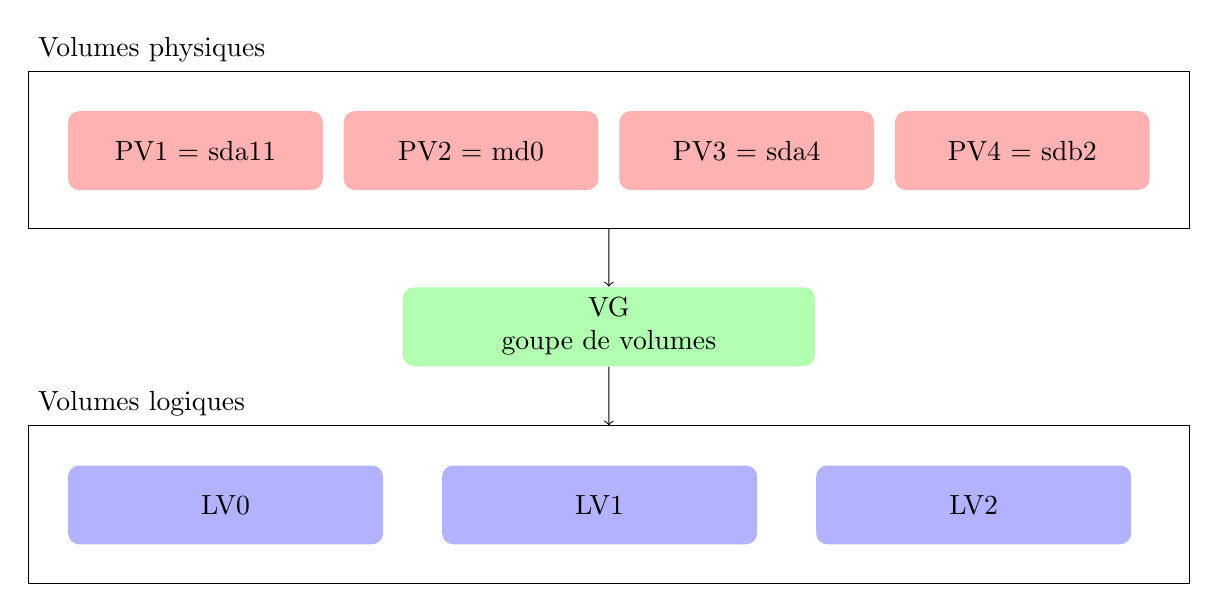
\begin{tikzpicture}

        \node (PV1) [incolore, anchor=north west, draw=none, fill=red!30] at (0,0) {PV1 = sda11};
        \node (PV2) [incolore, anchor=north west, draw=none, fill=red!30] at (3.5,0) {PV2 = md0};
        \node (PV3) [incolore, anchor=north west, draw=none, fill=red!30] at (7,0) {PV3 = sda4};
        \node (PV4) [incolore, anchor=north west, draw=none, fill=red!30] at (10.5,0) {PV4 = sdb2};
        \draw (-0.5,0.5) node[anchor=south west]{Volumes physiques} -- (14.25,0.5) -- (14.25,-1.5) -- (-0.5,-1.5) -- cycle;

        \node (VG) [incolore, anchor=south west, draw=none, fill=green!30, text width=5cm] at (4.25,-3.25) {VG \\ goupe de volumes};

        \node (LV0) [incolore, anchor=north west, draw=none, fill=blue!30, minimum width=4cm] at (0,-4.5) {LV0};
        \node (LV1) [incolore, anchor=north west, draw=none, fill=blue!30, minimum width=4cm] at (4.75,-4.5) {LV1};
        \node (LV2) [incolore, anchor=north west, draw=none, fill=blue!30, minimum width=4cm] at (9.5,-4.5) {LV2};

        \draw (-0.5,-4) node[anchor=south west]{Volumes logiques} -- (14.25,-4) -- (14.25,-6) -- (-0.5,-6) -- cycle;

        \draw[->] (13.75/2,-1.5) -- (VG);
        \draw[->] (VG) -- (13.75/2,-4);

    \end{tikzpicture}
\end{center}

\item Commandes:
\begin{itemize}
    \item lvmdiskscan : recherche les PV présents sur la machine
    \item vgscan : analyse tous les périphériques disques supportés dans le système afin de rechercher les volumes physiques LVM et les groupes de volumes. Cela permet de construire le fichier de cache LVM dans /etc/lvm/.cache, qui maintient une liste des périphériques LVM en cours.
    \item pvscan : recherche les volumes physiques à travers tous les périphériques blocs LVM supportés dans le système
    \item lvscan : scanne tous les VG connus ou tous les PV pris en charge dans le système pour déterminer le LV.
    \item pvcreate : Initialisation d’une partition ou d’un disque pour l’utiliser en LVM
    \item vgcreate : Création d’un groupe de volume
    \item lvcreate : Création d’un volume logique
    \item vgextend : Ajout d’une partition à un VG
    \item vgreduce : Suppression d’une partition à un VG
    \item lvextend : Permet d’augmenter la taille d’un LV
    \item lvreduce : Permet de réduire la taille d’un LV
    \item pvdisplay : Affiche les propriétés du volume physique
    \item vgdisplay : Affiche les propriétés du groupe de volume
    \item lvdisplay : Affiche les propriétés du volume logique
    \item lvremove : Supprime un LV. Les données sont perdues.
    \item vgremove : suppression d’un VG
    \item pvremove : Supression d’un PV
    \item pvmove : Déplacer des données présentent sur un PV vers un autre
\end{itemize}

\end{itemize}










\subsection{Manipulation - LVM}





\begin{itemize}

\item Créer 3 partitions LVM de 80, 160 et 240 Mo respectivement.
\begin{example}
    \begin{itemize}
        \item \texttt{sudo apt install lvm2}
        \item \texttt{sudo cfdisk} (mettre le type en : \textit{linux lvm})
    \end{itemize}
\end{example}

\item Créer les volumes physiques et vérifier leurs propriétés.
\begin{example}
    \begin{itemize}
        \item \texttt{sudo pvcreate -v /dev/sda\{12,13,14\}}
        \item \texttt{sudo pvdisplay} : Affiche les propriétés du volume physique
    \end{itemize}
\end{example}

\item Créer le groupe de volume VG0 et vérifier ses propriétés.
\begin{example}
    \begin{itemize}
        \item \texttt{sudo vgcreate -v <nom\_vg> <pv>}
        \item \texttt{sudo vgcreate -v vg0 /dev/sda\{12,13,14\}}
        \item \texttt{sudo vgdisplay} : Affiche les propriétés du groupe de volume
    \end{itemize}
\end{example}

\item Créer un volume logique de 120Mo et vérifier ses propriétés.
\begin{example}
    \begin{itemize}
        \item \texttt{lvcreate -n <nom\_LV> -L <taille> <vg>}
        \item \texttt{lvcreate -n lv0 -L 120M vg0}
        \item \texttt{sudo lvdisplay} : Affiche les propriétés du volume logique
    \end{itemize}
\end{example}

\item Le formater et le monter dans mnt.
\begin{example}
    \begin{itemize}
        \item \texttt{sudo mkfs.ext4 /dev/vg0/lv0}
        \item \texttt{sudo mount /dev/vg0/lv0 /mnt}
    \end{itemize}
\end{example}

\item Vérifier l'espace disponible sur le système de fichier.
\begin{example}
    \begin{itemize}
        \item \texttt{df /mnt} (df = disk free)
    \end{itemize}
\end{example}

\item Agrandir le volume logique de 50Mo.
\begin{example}
    \begin{itemize}
        \item \texttt{lvextend -L +50M /dev/vg0/lv0}
    \end{itemize}
\end{example}

\item Est-ce que l'espace disponible sur le système de fichier à changé ? \\
Pourquoi ? Si non, bien s'assurer que l'espace disponible est augmenté !
\begin{example}
    \begin{itemize}
        \item \texttt{df /mnt} (df = disk free)
        \item espace disponible sur le système de fichier = 104750 (inchangé)
        \item l'espace disponible sur le système de fichier n'a pas augmenté car on n'a pas utilisé la commande \texttt{resize2fs} pour l'agrandir
    \end{itemize}
\end{example}

\item Si l'on veut rétrécir un LV, dans quel ordre réaliser les étapes\footnote{https://www.tecmint.com/extend-and-reduce-lvms-in-linux/} ? Pourquoi ?
\begin{example}
    \begin{enumerate}
        \item démonter le système de fichiers
        \begin{itemize}
            \item \texttt{sudo umount /mnt}
        \end{itemize}
        \item vérifier le système de fichiers
        \begin{itemize}
            \item \texttt{e2fsck -ff /dev/vg0/lv0} (corrige les erreurs avec le journal)
        \end{itemize}
        \item réduire le système de fichiers
        \begin{itemize}
            \item \texttt{resize2fs /dev/vg0/lv0 10M}
        \end{itemize}
        \item réduire le volume logique (LV)
        \begin{itemize}
            \item \texttt{lvreduce -L -10M /dev/vg0/lv0}
        \end{itemize}
        \item re-vérifier le système de fichiers
        \begin{itemize}
            \item \texttt{e2fsck -ff /dev/vg0/lv0} (corrige les erreurs avec le journal)
        \end{itemize}
        \item remonter le système de fichiers
        \begin{itemize}
            \item \texttt{sudo mount /dev/vg0/lv0 /mnt}
        \end{itemize}
    \end{enumerate}
\end{example}

\item Supprimer le volume logique.
\begin{example}
    \begin{itemize}
        \item \texttt{sudo umount /mnt}
        \item \texttt{sudo lvremove vg0/lv0}
    \end{itemize}
\end{example}

\end{itemize}










\subsection{Manipulation - RAID + LVM}





\begin{itemize}

\item Le principe est identique à l’utilisation de disque simple (non RAID). Il faut au préalable créer le RAID (/dev/md0). Ensuite on l’utilise simplement comme PV : pvcreate /dev/md0.

\item Créer et tester un ensemble LVM par-dessus un ensemble raid. Vérifier.
\begin{example}
    \begin{itemize}
        \item \texttt{sudo pvcreate -v /dev/md0}
        \item \texttt{sudo vgcreate -v vg1 /dev/md0}
    \end{itemize}
\end{example}

\end{itemize}










\subsection{Manipulation avancées}





\begin{itemize}

\item Via fdisk créer 3 partitions de 300Mo
\begin{example}
    \begin{itemize}
        \item \texttt{sudo fdisk /dev/sda}
        \item commande = n
    \end{itemize}
\end{example}

\item Convertir la partition en ext2 (sda6) en ext3 et vérifier à nouveau
\begin{example}
    \begin{itemize}
        \item \texttt{sudo tune2fs -j /dev/sda6} (-j = ajouter la journalisation)
        \item \texttt{sudo mount /dev/sda6 /mnt}
        \item \texttt{stat -f /mnt}
    \end{itemize}
\end{example}

\item Rendre permanent le montage de la partition dans /mnt/test
\begin{itemize}
    \item Démonter sda6 : umount /dev/sda6
    \item Créer le répertoire test : mkdir /mnt/test
    \item Monter sda6 dans test : mount /dev/sda6 /mnt/test
\end{itemize}
\begin{example}
    \begin{itemize}
        \item \texttt{cp /etc/fstab f1}
        \item \texttt{sudo blkid /dev/sda6 >{}> f1} (pour obtenir l'uuid)
        \item \texttt{nano f1}, modifier la dernière ligne: \texttt{UUID=<uuid> /mnt/test ext3 defaults 0 0}
        \item \texttt{sudo cp f1 /etc/fstab}
    \end{itemize}
\end{example}

\item Lister les montages actifs
\begin{example}
    \begin{itemize}
        \item \texttt{mount}
    \end{itemize}
\end{example}

\item Vérifier l’espace libre/occupé sur les partitions montées
\begin{example}
    \begin{itemize}
        \item \texttt{df}
    \end{itemize}
\end{example}

\item Une fois la partition montée, vérifier si les fichiers présents auparavant sont effacés ou pas.
\begin{example}
    \begin{itemize}
        \item \texttt{ls /mnt/test}
    \end{itemize}
    Ils ne sont pas effacés.
\end{example}

\item Déplacer le répertoire home sur la partition ext4. Attention, travaillez de manière sécurisée ! Il ne faut pas risquer de perdre des données\footnote{https://www.tecmint.com/move-home-directory-to-new-partition-disk-in-linux/} !
\begin{example}
    \begin{enumerate}
        \item Créer la partition, le système de fichiers et la monter:
        \begin{itemize}
            \item \texttt{sudo cfdisk}, créer une partition de 2 Go
            \item \texttt{sudo mkfs.ext4 /dev/sda7}
            \item \texttt{sudo mount /dev/sda7 /mnt}
        \end{itemize}
        \item Copier les données de \texttt{/home} sur l'autre partition, puis les supprimer:
        \begin{itemize}
            \item \texttt{sudo cp -a /home/* /mnt/} (\texttt{-a} = copie récursive aussi proche que possible de l'original\footnote{Par exemple: \texttt{-a} ne change pas la date de modification, contrairement à \texttt{-r}. Plus d'informations sur: https://unix.stackexchange.com/a/44981})
            \item \texttt{sudo diff -r /home /mnt} (en cas de problème, supprimer puis recopier)
            \item \texttt{sudo rm -rf /home/*}
        \end{itemize}
        \item Démonter la partition puis la remonter sur \texttt{/home}:
        \begin{itemize}
            \item \texttt{sudo umount /mnt}
            \item \texttt{sudo mount /dev/sda7 /home}
        \end{itemize}
        \item Modifier l'UUID dans \texttt{/etc/fstab}:
        \begin{itemize}
            \item \texttt{cp /etc/fstab f1}
            \item \texttt{sudo blkid /dev/sda6 >{}> f1} (pour obtenir l’uuid)
            \item \texttt{nano f1}
            \begin{enumerate}
                \item commenter l'ancienne ligne avec \texttt{/home}
                \item modifier la dernière ligne: \texttt{UUID=<uuid> /home ext4 defaults 0 2}
            \end{enumerate}
            \item \texttt{sudo cp f1 /etc/fstab}
        \end{itemize}
        \item Vérification finale:
        \begin{itemize}
            \item \texttt{sudo reboot}
            \item \texttt{df -hl}
        \end{itemize}
    \end{enumerate}
\end{example}

\end{itemize}















\section{Network addressing services}










\subsection{Manipulation de base -- DNS}





\begin{itemize}

\item Install bind.
\begin{example}
    \begin{itemize}
        \item \texttt{sudo apt install bind9 bind9utils bind9-doc}
    \end{itemize}
\end{example}

\item DNS cache server.
\begin{example}
    Mettre la machine en NAT, puis changer la configuration dans \texttt{/etc/network/interfaces}:
    \begin{verbatim}
allow-hotplug enp0s3
iface enp0s3 inet static
    address 10.0.2.15
    netmask 255.255.255.0
    gateway 10.0.2.2
    dns-nameservers 127.0.0.1
    \end{verbatim}
    Commenter toutes les lignes dans \texttt{/etc/resolv.conf}. \\
\end{example}
\begin{example}
    \texttt{bind} est configuré en serveur dns cache par défaut.
    \begin{itemize}
        \item \texttt{nl /etc/bind/named.conf.options}
        \item paramètres:
        \begin{verbatim}
options {
    directory "/var/cache/bind";
    dnssec-validation auto;
    listen-on-v6 { any; };
};
        \end{verbatim}
    \end{itemize}
    En cas de modification du fichier (ex: pour ajouter un forwarder):
    \begin{itemize}
        \item \texttt{sudo named-checkconf -z} (vérifie la syntaxe des options)
        \item \texttt{sudo systemctl restart bind9}
        \item \texttt{sudo tail -f /var/log/syslog}
    \end{itemize}
    Ajouter: \texttt{nameserver <ip>}, dans: \texttt{/etc/network/interfaces}, la machine client.
\end{example}

\item Test bind as a cache server with nslookup.
\begin{example}
    \begin{itemize}
        \item \texttt{sudo apt install dnsutils}
        \item \texttt{nslookup fb.com}
        \item \texttt{nslookup fb.com} (ça devrait aller plus vite la 2ème fois)
        \item \texttt{nl /var/cache/bind/named\_dump.db} (contient le cache du serveur dns)
        \item \texttt{dig fb.com} (query time = 190 msec)
        \item \texttt{dig fb.com} (query time = 0 msec)
    \end{itemize}
\end{example}

\item Check and test the server configuration with:
\begin{itemize}
    \item \texttt{named-checkconf -z}
    \begin{example}
        Vérifier la syntaxe des fichiers de configuration:
        \begin{itemize}
            \item \texttt{sudo named-checkconf -z}
        \end{itemize}
    \end{example}
    \item \texttt{named-checkzone}
    \begin{example}
        Vérifie la validité du fichier de zones:
        \begin{itemize}
            \item \texttt{sudo named-checkzone [<fichier\_conf> | <domaine.com> <fichier\_zone>]}
            \item \texttt{sudo named-checkzone /etc/bind/named.conf}
        \end{itemize}
    \end{example}
    \item \texttt{nslookup}
    \item \texttt{dig}
    \begin{example}
        \begin{itemize}
            \item \texttt{dig fb.com}
        \end{itemize}
    \end{example}
    \item \texttt{host}
    \begin{example}
        \begin{itemize}
            \item \texttt{host fb.com}
        \end{itemize}
    \end{example}
\end{itemize}

\item Create a primary dns zone "myname.linux".
\begin{itemize}
    \item Don't forget the reverse zone !
    \item Tip : start from the db.empty file !
\end{itemize}
\begin{example}

Fichier \texttt{/etc/bind/named.conf.local}:
\begin{verbatim}
    zone "myname.linux" {
        type master;
        file "/etc/bind/db.myname.linux";
    };

    // 10.0.2.15
    zone "2.0.10.in-addr.arpa" {
        type master;
        file "/etc/bind/db.myname.linux.inv";
    };
\end{verbatim}

Fichier \texttt{/etc/bind/db.myname.linux}:
\begin{verbatim}
    $TTL    86400
    @       IN      SOA     myname.linux.    root.myname.linux. (
                            1           ; Serial
                            604800      ; Refresh
                            86400       ; Retry
                            2419200     ; Expire
                            86400       ; Negative Cache TL
                            )

    @       IN      NS      myname.linux.
            IN      A       10.0.2.15
    dns     IN      CNAME   myname.linux.
    www     IN      CNAME   myname.linux.
\end{verbatim}

Fichier \texttt{/etc/bind/db.myname.linux.inv}:
\begin{verbatim}
    $TTL    86400
    @       IN      SOA     myname.linux.    root.myname.linux. (
                            1           ; Serial
                            604800      ; Refresh
                            86400       ; Retry
                            2419200     ; Expire
                            86400       ; Negative Cache TL
                            )

    @       IN      NS      myname.linux.
    15      IN      PTR     myname.linux
    15      IN      PTR     dns.myname.linux
    15      IN      PTR     www.myname.linux
\end{verbatim}

Vérifications:
\begin{itemize}
    \item \texttt{sudo named-checkconf -z} (vérifie la syntaxe des options)
    \item \texttt{sudo named-checkzone myname.linux /etc/bind/db.myname.linux}
    \item \texttt{sudo named-checkzone 10.in-addr.arpa /etc/bind/db.myname.linux.inv}
    \item \texttt{sudo systemctl restart bind9}
    \item \texttt{sudo tail /var/log/syslog}
    \item \texttt{nslookup www.myname.linux}
    \item \texttt{nslookup dns.myname.linux}
    \item \texttt{nslookup myname.linux}
    \item \texttt{nslookup 10.0.2.15}
\end{itemize}

\end{example}

\item Add an MX, an A and a CNAME record.
\begin{itemize}
    \item Don’t forget good practices: ONE A record for each IP! Others $ \rightarrow $ CNAME.
    \item MX record is for a zone, not for an host!
    \item Don’t forget to check and test the server configuration!
\end{itemize}
\begin{example}
Fichier \texttt{/etc/bind/db.myname.linux}:
\begin{verbatim}
    $TTL    86400
    @       IN      SOA     myname.linux.    root.myname.linux. (
                            1           ; Serial
                            604800      ; Refresh
                            86400       ; Retry
                            2419200     ; Expire
                            86400       ; Negative Cache TL
                            )

    @       IN      NS      myname.linux.
    @       IN      MX      10 myname.linux.
            IN      A       10.0.2.15
    dns     IN      CNAME   myname.linux.
    www     IN      CNAME   myname.linux.
    mail    IN      CNAME   myname.linux.
\end{verbatim}
Ça revient à ajouter la ligne avec le MX, et la ligne avec mail en CNAME.
\end{example}

\item Create the corresponding reverse zones and PTR records.
\begin{example}
Fichier \texttt{/etc/bind/db.myname.linux.inv}:
\begin{verbatim}
    $TTL    86400
    @       IN      SOA     myname.linux.    root.myname.linux. (
                            1           ; Serial
                            604800      ; Refresh
                            86400       ; Retry
                            2419200     ; Expire
                            86400       ; Negative Cache TL
                            )

    @       IN      NS      myname.linux.
    15      IN      PTR     myname.linux
    15      IN      PTR     dns.myname.linux
    15      IN      PTR     www.myname.linux
    15      IN      PTR     mail.myname.linux
\end{verbatim}
\end{example}

\item Don’t forget to check and test.
\begin{example}
    Vérifier l'enregistrement MX:
    \begin{itemize}
        \item \texttt{nslookup mail.myname.linux}
        \item \texttt{nslookup}
        \item \texttt{set q=MX}
        \item \texttt{myname.linux}
    \end{itemize}
\end{example}

\end{itemize}










\subsection{Autre configuration DNS}





\begin{itemize}

\item Fichier \texttt{/etc/bind/db.myname.linux}:
\begin{example} \begin{verbatim}
$TTL    86400
@       IN      SOA     srv.myname.linux.    root.myname.linux. (
                        1           ; Serial
                        604800      ; Refresh
                        86400       ; Retry
                        2419200     ; Expire
                        86400       ; Negative Cache TL
                        )

@       IN      NS      srv.myname.linux.
@       IN      MX      10 srv
        IN      A       10.0.2.15
dns     IN      CNAME   srv
www     IN      CNAME   srv
mail    IN      CNAME   srv
\end{verbatim} \end{example}

\item Fichier \texttt{/etc/bind/db.myname.linux.inv}:
\begin{example} \begin{verbatim}
$TTL    86400
@       IN      SOA     srv.myname.linux.    root.myname.linux. (
                        1           ; Serial
                        604800      ; Refresh
                        86400       ; Retry
                        2419200     ; Expire
                        86400       ; Negative Cache TL
                        )

@       IN      NS      srv.myname.linux.
15      IN      PTR     srv
15      IN      PTR     srv
15      IN      PTR     srv
15      IN      PTR     srv
\end{verbatim} \end{example}

\end{itemize}










\subsection{Manipulation de base -- DHCP}





\begin{itemize}

\item Install the dhcp server.
\begin{example}
    \begin{itemize}
        \item \texttt{sudo apt install isc-dhcp-server}
    \end{itemize}
    \textbf{Remarques}:
    \begin{itemize}
        \item perso, quand je reboot, le serveur ne fonctionne plus mais ça ne marque rien dans le journal
        \item il faut redémarrer le service avec: \texttt{systemctl restart isc-dhcp-server}
        \item mais avant, il faut que l'interface sur laquelle le service est configuré soit up (\texttt{ifup <interface>})
    \end{itemize}
\end{example}

\item Study a few configuration file’s included examples.
\begin{example}
    \begin{itemize}
        \item \texttt{ls /etc/dhcp}
        \item \texttt{cat /etc/dhcp/dhcpd.conf}
    \end{itemize}
\end{example}

\item By default, the service is not working. Check in the logs why!
\begin{example}
    \begin{itemize}
        \item \texttt{journalctl -xe}
        \item \texttt{tail /var/log/syslog}
        \item \texttt{tail f /var/log/syslog} (pour afficher en continu)
    \end{itemize}
\end{example}

\item Activate the service. Be careful!
\begin{itemize}
    \item Do it on the right interface.
    \item Configure it to work on the NIC that is not plugged to the iesn network. Why? $ \implies $ only one DHCP/LAN.
\end{itemize}
\begin{example}
    Ajouter l'interface:
    \begin{itemize}
        \item \texttt{sudo nano /etc/default/isc-dhcp-server}
        \item ajouter \texttt{enp0s8} aux interfaces en ipv4
    \end{itemize}
    \textbf{Remarque}: les interfaces dans virtualbox sont:
    \begin{itemize}
        \item \texttt{enp0s3} = en NAT
        \item \texttt{enp0s8} = en réseau interne
    \end{itemize}
    Configurer le dhcpd:
    \begin{itemize}
        \item \texttt{sudo nano /etc/dhcp/dhcpd.conf}
        \item modifier:
        \begin{verbatim}
    authoritative;

    subnet 192.168.0.0 netmask 255.255.255.0 {
        option routers 192.168.0.1;
        range 192.168.0.2 192.168.0.254;
        option broadcast-address 192.168.0.255;
    }
        \end{verbatim}
    \end{itemize}
    Tester la config:
    \begin{itemize}
        \item \texttt{sudo systemctl restart isc-dhcp-server}
        \item \texttt{sudo tail -f /var/log/syslog}
        \item lancer la 2ème machine en dhcp dans le réseau interne
    \end{itemize}
    \textbf{Remarque}: L'interface enp0s8 doit être configurée en statique car elle ne peut pas recevoir de configuration sinon.
\end{example}

\item Check in the file the default lease time.
\begin{example}
    Ouvrir le fichier:
    \begin{itemize}
        \item \texttt{sudo nano /etc/dhcp/dhcpd.conf}
    \end{itemize}
    Les configs de lease time sont:
    \begin{verbatim}
default-lease-time 600;
max-lease-time 7200;
    \end{verbatim}
\end{example}

\item Don't forget to configure the right values (choose DNS values from the previous labs) for:
\begin{itemize}
    \item the netmask,
    \item the IP address range,
    \item the name servers,
    \item the gateway,
    \item the search domain,
    \item the ntp server,
    \item etc.
\end{itemize}
\begin{example}
\begin{verbatim}
# /etc/dhcp/dhcpd.conf
subnet 192.168.0.0 netmask 255.255.255.0 {      # netmask
    range 192.168.0.2 192.168.0.254;            # ip range
    option domain-name-servers 192.168.0.1;     # dns
    option routers 192.168.0.1;                 # gateway
    option domain-search "myname.linux";        # search domain
    option ntp-servers 192.168.0.1;             # ntp
    option broadcast-address 192.168.0.255; # pas obligatoire
}
\end{verbatim}
\textbf{Remarque}: il faut que le ntp et le dns soient installés.
\begin{itemize}
    \item dans \texttt{/etc/ntp.conf}, ajouter: \texttt{restrict 192.168.0.0 mask 255.255.255.0}
\end{itemize}
\end{example}

\item Test it using one of the lab's switches (or a cross cable) and with your neighbour’s computer as a client, or with a Live CD VM.
\begin{example}
    Vérifications sur la machine cliente:
    \begin{itemize}
        \item \texttt{ip a} (ip + netmask)
        \item \texttt{ip route} (gateway)
        \item \texttt{cat /etc/resolv.conf} (dns + search domain)
        \item \texttt{ntptrace} (ntp)
    \end{itemize}
\end{example}

\item Configure the server so that it always gives the client the same IP (a fixed lease).
\begin{example}
\begin{verbatim}
host client_fixed_ip {
    hardware ethernet 08:00:07:26:c0:a5;
    fixed-address 192.168.0.2;
}
\end{verbatim}
\end{example}

\end{itemize}










\subsection{Manipulation avancée}





\begin{itemize}

\item Create a secondary dns zone with your neighbour as the primary zone, and reciprocally.
\begin{center}
    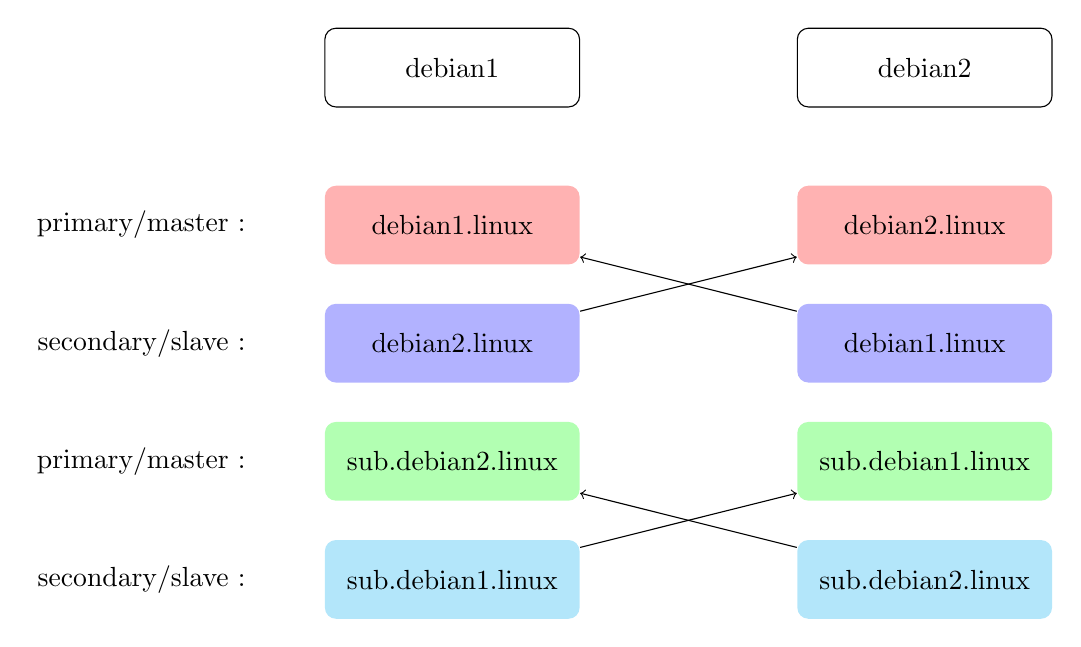
\begin{tikzpicture}
        \node (d1) [incolore] at (0,0) {debian1};
        \node (d2) [incolore] at (6,0) {debian2};

        \node () [anchor=east] at (-2.5,-2.0) {primary/master :};
        \node () [anchor=east] at (-2.5,-3.5) {secondary/slave :};
        \node () [anchor=east] at (-2.5,-5.0) {primary/master :};
        \node () [anchor=east] at (-2.5,-6.5) {secondary/slave :};
        
        \node (d11) [incolore, draw=none, fill=red!30]   at (0,-2.0) {debian1.linux};
        \node (d21) [incolore, draw=none, fill=red!30]   at (6,-2.0) {debian2.linux};
        \node (d12) [incolore, draw=none, fill=blue!30]  at (0,-3.5) {debian2.linux};
        \node (d22) [incolore, draw=none, fill=blue!30]  at (6,-3.5) {debian1.linux};
        \node (d13) [incolore, draw=none, fill=green!30] at (0,-5.0) {sub.debian2.linux};
        \node (d23) [incolore, draw=none, fill=green!30] at (6,-5.0) {sub.debian1.linux};
        \node (d14) [incolore, draw=none, fill=cyan!30]  at (0,-6.5) {sub.debian1.linux};
        \node (d24) [incolore, draw=none, fill=cyan!30]  at (6,-6.5) {sub.debian2.linux};

        \draw[->] (d12) -- (d21);
        \draw[->] (d22) -- (d11);
        \draw[->] (d14) -- (d23);
        \draw[->] (d24) -- (d13);
    \end{tikzpicture}
\end{center}
\begin{example}
    debian1:
    \begin{itemize}
        \item Fichier \texttt{/etc/network/interfaces}:
        \begin{verbatim}
    allow-hotplug enp0s8
    iface enp0s3 inet static
        address 192.168.0.1
        netmask 255.255.255.0
        gateway 192.168.0.1
        dns-nameservers 192.168.0.1 192.168.0.2
        \end{verbatim}
        \item Fichier \texttt{/etc/bind/named.conf.local}:
        \begin{verbatim}
    zone "debian1.linux" {
        type master;
        file "/etc/bind/db.debian1.linux";
    };
    // 192.168.0.1
    zone "1.0.168.192.in-addr.arpa" {
        type master;
        file "/etc/bind/db.debian1.linux.inv";
    };

    zone "debian2.linux" {
        type slave;
        masters { 192.168.0.2; };
    };
    // 192.168.0.2
    zone "2.0.168.192.in-addr.arpa" {
        type slave;
        masters { 192.168.0.2; };
    };
        \end{verbatim}
        \item Fichier \texttt{/etc/bind/db.debian1.linux}:
        \begin{verbatim}
    $TTL    86400
    @       IN      SOA     debian1.linux.    root.debian1.linux. (
                            1           ; Serial
                            604800      ; Refresh
                            86400       ; Retry
                            2419200     ; Expire
                            86400       ; Negative Cache TL
                            )

    @       IN      NS      debian1.linux.
            IN      A       192.168.0.1
    www     IN      CNAME   debian1.linux.
        \end{verbatim}
        \item Fichier \texttt{/etc/bind/db.debian1.linux.inv}:
        \begin{verbatim}
    $TTL    86400
    @       IN      SOA     debian1.linux.    root.debian1.linux. (
                            1           ; Serial
                            604800      ; Refresh
                            86400       ; Retry
                            2419200     ; Expire
                            86400       ; Negative Cache TL
                            )

    @       IN      NS      debian1.linux.
            IN      PTR     debian1.linux
            IN      PTR     www.debian1.linux
        \end{verbatim}
    \end{itemize}
    debian2:
    \begin{itemize}
        \item Fichier \texttt{/etc/network/interfaces}:
        \begin{verbatim}
    allow-hotplug enp0s3
    iface enp0s3 inet dhcp
        \end{verbatim}
        \item Fichier \texttt{/etc/bind/named.conf.local}:
        \begin{verbatim}
    zone "debian2.linux" {
        type master;
        file "/etc/bind/db.debian1.linux";
    };
    // 192.168.0.2
    zone "2.0.168.192.in-addr.arpa" {
        type master;
        file "/etc/bind/db.debian2.linux.inv";
    };

    zone "debian1.linux" {
        type slave;
        masters { 192.168.0.1; };
    };
    // 192.168.0.1
    zone "1.0.168.192.in-addr.arpa" {
        type slave;
        masters { 192.168.0.1; };
    };
        \end{verbatim}
        \item Fichier \texttt{/etc/bind/db.debian2.linux}:
        \begin{verbatim}
    $TTL    86400
    @       IN      SOA     debian2.linux.    root.debian2.linux. (
                            1           ; Serial
                            604800      ; Refresh
                            86400       ; Retry
                            2419200     ; Expire
                            86400       ; Negative Cache TL
                            )

    @       IN      NS      debian2.linux.
            IN      A       192.168.0.2
    www     IN      CNAME   debian2.linux.
        \end{verbatim}
        \item Fichier \texttt{/etc/bind/db.debian2.linux.inv}:
        \begin{verbatim}
    $TTL    86400
    @       IN      SOA     debian2.linux.    root.debian2.linux. (
                            1           ; Serial
                            604800      ; Refresh
                            86400       ; Retry
                            2419200     ; Expire
                            86400       ; Negative Cache TL
                            )

    @       IN      NS      debian2.linux.
            IN      PTR     debian2.linux
            IN      PTR     www.debian2.linux
        \end{verbatim}
    \end{itemize}
    \textcolor{red}{\textbf{Attention !}} Pas besoin de donner des fichiers dans les zones esclaves.
\end{example}

\item Don’t forget to check and test.
\begin{example}
    \begin{itemize}
        \item \texttt{sudo systemctl restart bind9}
        \item \texttt{nslookup www.debian1.linux}
        \item \texttt{nslookup www.debian2.linux}
    \end{itemize}
\end{example}

\item Add the secondary DNS to your DHCP’s configuration file.
\begin{example}
    Fichier \texttt{/etc/dhcp/dhcpd.conf}:
    \begin{verbatim}
    subnet 192.168.0.0 netmask 255.255.255.0 {
        # modifier cette option:
        option domain-name-server 192.168.0.1, 192.168.0.2;
    }
    \end{verbatim}
\end{example}

\item Only your secondary zone is allowed to ask for updates. Only your primary zone is allowed to send updates to your secondary one.
\begin{itemize}
    \item allow-notify = slave, by default only master can update
    \item allow-transfer = master, by default anybody can take update
\end{itemize}
\begin{example}
    Les modifications doivent être réalisées dans les points suivants.
\end{example}

\item Queries are only authorized for your domains.
\begin{example}
    Fichier \texttt{/etc/bind/named.conf.options}:
    \begin{verbatim}
    options {
        // ajouter l'option suivante:
        allow-notify { 192.168.0.0; };
    }
    \end{verbatim}
\end{example}

\item Hosts from your lan can queries for external domains too.
\begin{example}
    Fichier \texttt{/etc/bind/named.conf.options}:
    \begin{verbatim}
    options {
        // ajouter l'option suivante:
        allow-transfer { 192.168.0.0; };
    }
    \end{verbatim}
\end{example}

\item Create a sub domain called "sub.debian1.linux.". This domain is delegated to a new zone managed by your neighbor’s DNS service.
\begin{example}
    Debian1:
    \begin{itemize}
        \item Fichier \texttt{/etc/bind/named.conf.local}:
        \begin{verbatim}
    zone "sub.debian1.linux" {
        type slave;
        masters { 192.168.0.2; };
    };
        \end{verbatim}
    \end{itemize}
    Debian2:
    \begin{itemize}
        \item Fichier \texttt{/etc/bind/named.conf.local}:
        \begin{verbatim}
    zone "sub.debian1.linux" {
        type master;
        file "/etc/bind/db.sub.debian1.linux";
    };
        \end{verbatim}
        \item Fichier \texttt{/etc/bind/db.sub.debian1.linux}:
        \begin{verbatim}
    $TTL    86400
    @       IN      SOA     sub.debian1.linux.    root.sub.debian1.linux. (
                            1           ; Serial
                            604800      ; Refresh
                            86400       ; Retry
                            2419200     ; Expire
                            86400       ; Negative Cache TL
                            )

    @       IN      NS      sub.debian1.linux.
    ; j'ai laissé l'ip de debian1, mais on s'en fiche
            IN      A       192.168.0.1
    www     IN      CNAME   sub.debian1.linux.
        \end{verbatim}
    \end{itemize}
\end{example}

\item Create a zone "sub.debian2.linux". This zone manages your neighbor sub domain.
\begin{example}
    Debian1:
    \begin{itemize}
        \item Fichier \texttt{/etc/bind/named.conf.local}:
        \begin{verbatim}
    zone "sub.debian2.linux" {
        type master;
        file "/etc/bind/db.sub.debian2.linux";
    };
        \end{verbatim}
        \item Fichier \texttt{/etc/bind/db.sub.debian2.linux}:
        \begin{verbatim}
    $TTL    86400
    @       IN      SOA     sub.debian2.linux.    root.sub.debian2.linux. (
                            1           ; Serial
                            604800      ; Refresh
                            86400       ; Retry
                            2419200     ; Expire
                            86400       ; Negative Cache TL
                            )

    @       IN      NS      sub.debian2.linux.
    ; j'ai laissé l'ip de debian2, mais on s'en fiche
            IN      A       192.168.0.2
    www     IN      CNAME   sub.debian2.linux.
        \end{verbatim}
    \end{itemize}
    Debian2:
    \begin{itemize}
        \item Fichier \texttt{/etc/bind/named.conf.local}:
        \begin{verbatim}
    zone "sub.debian2.linux" {
        type slave;
        masters { 192.168.0.1; };
    };
        \end{verbatim}
    \end{itemize}
\end{example}

\begin{center}
    \textcolor{blue}{\textbf{LE RESTE DE CETTE MANIP EST OPTIONNEL}}
\end{center}

\item Notes:
\begin{itemize}
    \item It's possible to dynamically update the DNS database with the DHCP server (Like in the AD).
    \item To do that, it's necessary to modify bind et dhcpd configuration.
\end{itemize}

\item Modify the dns et dhcp server configuration file to activate DynDNS.
\begin{example}
    http://www.linux-france.org/prj/edu/archinet/systeme/ch37.html
\end{example}

\item Secure the exchange of information between the servers
\begin{itemize}
    \item manual key or dnssec-keygen -a HMAC-MD5 -b 128 -r /dev/urandom -n USER DDNS\_UPDATE
    \item \begin{verbatim}
key DDNS_UPDATE {
    algorithm HMAC-MD5.SIG-ALG.REG.INT;
    secret "<key>";
};
    \end{verbatim}
    \item \begin{verbatim}
include "/etc/bind/ddns.key";

zone "example.org" {
    type master;
    notify no;
    file "/var/cache/bind/db.example.org";
    allow-update { key DDNS_UPDATE; };
};

zone "2.168.192.in-addr.arpa" {
    type master;
    notify no;
    file "/var/cache/bind/db.192.168.2";
    allow-update { key DDNS_UPDATE; };
};
    \end{verbatim}
    \item !!!!! : file permissions for bind to read/updates zone files!
    \item \begin{verbatim}
DHCP:ddns-updates on;

ddns-update-style      interim;
ignore                 client-updates;
update-static-leases   on;
    \end{verbatim}
    \item \begin{verbatim}
include "/etc/dhcp/ddns.key";
zone example.org. {
    primary 127.0.0.1;
    key DDNS_UPDATE;
}

zone 2.168.192.in-addr.arpa. {
    primary 127.0.0.1;
    key DDNS_UPDATE;
}
    \end{verbatim}
\end{itemize}

\item Your neighbor will be the DHCP and the DNS client.

\item Configure the client to use the hostname "my\_firstname". sudo vi /etc/dhcp3/dhclient.conf.

\item Set hostname as follows: send host-name "smlfkjqmflkjmlkjfqmlkfsdj";

\end{itemize}















\section{Démarrage, initialisation, gestion des processus}










\subsection{Le chargeur de démarrage}





À l’écran du GRUB, passer en mode édition et modifier la ligne linux
\begin{example}
    \begin{enumerate}
        \item au démarrage, à l'écran du GRUB, taper sur la touche \textit{e}
        \item modifier la 3ème ligne en partant par la fin dans l'éditeur:
        \begin{itemize}
            \item modifier \textit{ro}, en \textit{rw}
            \item ajouter \textit{init=/bin/bash} à la fin de la ligne
        \end{itemize}
        \item lancer la machine, en appuyant sur \textit{ctrl+x} ou \textit{f10}
        \item modifier le mot de passe (\texttt{passwd}, attention ! clavier en qwerty)
        \item taper : \texttt{sync}, taper : \texttt{exec /sbin/init}
        \item relancer la machine : \texttt{reboot}
    \end{enumerate}
\end{example}
Tester le nouveau mot de passe.










\subsection{Systemd}





\begin{itemize}

\item Installez Bind9.
\begin{example}
    \begin{itemize}
        \item \texttt{sudo apt install bind9}
    \end{itemize}
\end{example}

\item Vérifiez le statut du service bind9.
\begin{example}
    \begin{itemize}
        \item \texttt{sudo systemctl status bind9}
    \end{itemize}
\end{example}

\item Vérifiez que le service bind9 est une dépendance de multi-user.target.
\begin{example}
    \begin{itemize}
        \item \texttt{sudo systemctl list-dependencies -{}-after multi-user.target}
    \end{itemize}
\end{example}

\item Rebootez et vérifiez à nouveau le statut de bind9.
\begin{example}
    \begin{itemize}
        \item \texttt{reboot}
        \item \texttt{sudo systemctl list-dependencies -{}-after multi-user.target}
    \end{itemize}
\end{example}

\item Supprimez la dépendance de bind9 à multi-user.target.
\begin{example}
    \begin{itemize}
        \item \texttt{sudo systemctl disable bind9}
    \end{itemize}
\end{example}

\item Rebootez et vérifiez à nouveau le statut de bind9.
\begin{example}
    \begin{itemize}
        \item \texttt{reboot}
        \item \texttt{sudo systemctl status bind9}
    \end{itemize}
\end{example}

\item Pouvez vous néanmoins démarrer le service ?
\begin{example}
    Si on l'a masqué, non. Sinon je ne sais pas.
\end{example}

\item Effectuez les modifications nécessaire pour empêcher le démarrage de bind9.
\begin{example}
    \begin{itemize}
        \item \texttt{sudo systemctl mask bind9}
    \end{itemize}
\end{example}

\end{itemize}










\subsection{Gestion des processus}





\begin{itemize}

\item Lister les processus dont vous êtes le propriétaire qui sont attachés à votre console.
\begin{example}
    \begin{itemize}
        \item \texttt{ps -{}-user <user>}
    \end{itemize}
\end{example}

\item Lister l'entièreté de vos processus.
\begin{example}
    \begin{itemize}
        \item \texttt{ps -e}
    \end{itemize}
\end{example}

\item Lister tous les processus en cours d’exécution.
\begin{example}
    \begin{itemize}
        \item \texttt{ps -aux}
    \end{itemize}
\end{example}

\item Lister les processus sous forme d'un arbre.
\begin{example}
    \begin{itemize}
        \item \texttt{ps -e -{}-forest}
    \end{itemize}
\end{example}

\item Quelle est la particularité du processus 1?
\begin{example}
    C'est toujours \texttt{systemd}.
\end{example}

\item Si vous lancez 10 fois un programme, est-ce que le PID restera le même?
\begin{example}
    Non. Ça change à chaque fois.
\end{example}

\item Listez en continu les processus, en les triant par :
\begin{itemize}
    \item \%CPU
    \item \%mémoire
    \item Temps CPU
    \item top
\end{itemize}
\begin{example}
    \begin{itemize}
        \item \texttt{top -o \%CPU}
        \item \texttt{top -o \%MEM}
        \item \texttt{top -o TIME+}
        \item \texttt{ps -aux -{}-sort=cpu,mem,time}
    \end{itemize}
\end{example}

\item Trouver son numéro de processus via les commandes:
\begin{itemize}
    \item ps
    \item pgrep
\end{itemize}
\begin{example}
    \begin{itemize}
        \item \texttt{ps -aux | egrep bind}
    \end{itemize}
\end{example}

\item Lancer Firefox avec la plus faible priorité possible. Vérifier la priorité reçue.
\begin{example}
    \begin{itemize}
        \item \texttt{nice -20 firefox \&}
    \end{itemize}
\end{example}

\item Modifier la priorité de Firefox à la plus petite priorité possible. Vérifier la priorité reçue.
\begin{example}
    \begin{itemize}
        \item \texttt{ps -l}
        \item \texttt{renice -20 <PID\_firefox>}
    \end{itemize}
\end{example}

\item Consulter sa page de manuel si besoin et le lancer en avant plan, à des fin de "debug" par exemple:
\begin{itemize}
    \item man named
    \item -d (debug) -g (foreground + messages)
\end{itemize}

\item Le tester avec nslookup.
\begin{example}
    \begin{itemize}
        \item \texttt{named -d}
        \item \texttt{named -g}
    \end{itemize}
\end{example}

\item Mettre bind en pause.
\begin{example}
    \begin{itemize}
        \item \texttt{jobs -l}
        \item \texttt{kill -STOP \%<job\_id>}
    \end{itemize}
\end{example}

\item Le relancer en avant plan.
\begin{example}
    \begin{itemize}
        \item \texttt{fg <jobid>} (fg = foreground)
    \end{itemize}
\end{example}

\item Tuer bind.
\begin{example}
    \begin{itemize}
        \item \texttt{kill bind9}
    \end{itemize}
\end{example}

\item Quelle est la "procédure" standard pour relancer bind ? Analyser le script qui gère bind.
\begin{example}
    \begin{itemize}
        \item \texttt{kill -START \%<job\_id>}
    \end{itemize}
\end{example}

\item À l'aide de cron, faites redémarrer votre machine tout les jours à la même heure.
\begin{example}
    \begin{itemize}
        \item \texttt{at <heures>:<minutes>}
        \item \texttt{commande}
        \item \textit{ctrl+d}
    \end{itemize}
    \textbf{Remarque}: vérifier l'heure avec la commande : \texttt{date} (au cas où la machine n'est pas à l'heure belge).
\end{example}

\item Créer un script qui redémarre votre machine. Lancez-le dans quelques instants à l'aide de at.
\begin{example}
    \begin{itemize}
        \item \texttt{at <heures>:<minutes> -f <fichier>}
    \end{itemize}
\end{example}

\item Vérifiez que votre script est en attente d'exécution.
\begin{example}
    \begin{itemize}
        \item \texttt{atq}
    \end{itemize}
\end{example}

\end{itemize}










\subsection{Gestion des modules kernel}





\begin{itemize}

\item Lister les modules kernel utilisés.
\begin{example}
    \begin{itemize}
        \item \texttt{lsmod}
    \end{itemize}
\end{example}

\item Vérifier que le module vfat est désactivé. Sinon le désactiver.
\begin{example}
    \begin{itemize}
        \item \texttt{modinfo vfat}
    \end{itemize}
\end{example}

\item Monter un système de fichier vfat (partition, clef usb, etc.).
\begin{example}
    \begin{itemize}
        \item \texttt{mount -t vfat <partition> <dossier>}
    \end{itemize}
\end{example}

\item Lister les modules. Que constatez-vous? Qu'en conclure?
\begin{example}
    \begin{itemize}
        \item \texttt{lsmod}
    \end{itemize}
\end{example}

\item Récupérer les informations du modules reiserfs.
\begin{example}
    \begin{itemize}
        \item \texttt{modinfo reiserfs}
    \end{itemize}
\end{example}

\item Activer le module reiserfs et vérifier.
\begin{example}
    \begin{itemize}
        \item \texttt{insmod /lib/modules/4.19.0-12-amd64/kernel/fs/reiserfs/reiserfs.ko}
        \item \texttt{lsmod | grep reiserfs}
    \end{itemize}
\end{example}

\end{itemize}










\subsection{PAM}





\begin{itemize}

\item Grâce à Pam, permettre la création automatique du répertoire personnel des utilisateurs qui n'en auraient pas. Tester.
\begin{example}
    Ajouter un utilisateur qui n'a pas de répertoire personnel:
    \begin{itemize}
        \item \texttt{useradd test1}
        \item \texttt{passwd test1}
    \end{itemize}
    Dans le fichier \texttt{/etc/pam.d/login}, ajouter:
    \begin{verbatim}
session required pam_mkhomedir.so
    \end{verbatim}
    Relancer la machine et se connecter avec l'utilisateur qui n'a pas de répertoire personnel.
\end{example}
\textbf{Remarque}: il faut mettre les lignes de session vers la fin, sinon la machine risque de refuser toutes les sessions (impossible de se connecter).
\begin{center}
    \includegraphics[width=0.75\linewidth]{images/002.PNG}
\end{center}

\item Modifier le nombre d'essais de saisie d'un nouveau mot de passe à 2. Créer une stratégie de mot de passes qui force une longueur minimale, etc.
\begin{example}
    Dans le fichier \texttt{/etc/pam.d/login}, ajouter:
    \begin{verbatim}
session required pam_tally.so deny=2
session required pam_unix.so  minlen=6
    \end{verbatim}
\end{example}

\item Créer un utilisateur "pam". Pour ce dernier, interdire la connexion durant une courte tranche horaire. Vérifier.
\begin{example}
    \begin{itemize}
        \item \texttt{adduser pam}
        \item \texttt{nano /etc/pam.d/login}
        \item modifier:
        \begin{verbatim}
# interdiction de 10 sec
session required pam_tally.so deny=2 lock_time=10
        \end{verbatim}
        \item se connecter sur le compte avec un mauvais mot de passe à 2 reprises
    \end{itemize}
\end{example}

\end{itemize}















\section{Serveur WEB}










\subsection{Concepts}





\begin{itemize}

\item Installer un navigateur en ligne de commande, pratique pour tester nos configurations quand on a pas d’interface graphique:
\begin{itemize}
    \item \texttt{sudo apt install w3m w3m-img}
\end{itemize}

\item Visiter \textit{www.google.com}:
\begin{itemize}
    \item \texttt{w3m www.google.com}
\end{itemize}

\item Installer le service http apache:
\begin{itemize}
    \item \texttt{sudo apt install apache2}
\end{itemize}

\item Tester avec le navigateur w3m en ligne de commande:
\begin{itemize}
    \item \texttt{w3m 127.0.0.1}
\end{itemize}

\item Tester avec un navigateur graphique.

\item Les paramètres généraux d'apache sont stockés dans le fichier \textit{/etc/apache2/apache2.conf}.

\item Les ports d'écoute sont configurés dans le fichier \textit{/etc/apache2/ports.conf}.
\begin{itemize}
    \item par défaut, le port 80 est utilisé
    \item si il y a plusieurs ip, on peut associer port et ip : \texttt{Listen 192.168.0.1:80}
\end{itemize}

\item Chaque site possède son fichier de configuration que l’on peut "activer". Ils se trouvent dans le répertoire : \textit{/etc/apache2/sites-available}.

\item Ajouter la ligne suivante dans le fichier de configuration principal:
\begin{verbatim}
IncludeOptionnal sites-enabled/*.conf
\end{verbatim}
Pour activer un site, il suffit de créer un lien dans le répertoire \textit{/etc/apache2/sites-enabled} vers le fichier de configuration dans le répertoire \textit{/etc/apache2/sites-available}.

\item Exemple configuration \textit{/etc/apache2/sites-availbale/apache.local.conf}:
\begin{verbatim}
<VirtualHost 192.168.0.1:80>
    ServerName www.apache.local
    ServerAdmin webmaster@apache.local
    DocumentRoot /var/www/html/apache.local/
    ErrorLog ${APACHE_LOG_DIR}/apache.local.error.log
    CustomLog ${APACHE_LOG_DIR}/apache.local.access.log combined
</VirtualHost>
\end{verbatim}

\item Le protocole HTTPS est basé sur deux technologies :
\begin{itemize}
    \item le cryptage asymétrique (clé publique / clé privée)
    \item la certification numérique X509
\end{itemize}

\item Générer une clé de chiffrement et un certificat:
\begin{itemize}
    \item \texttt{openssl req -x509 -nodes -newkey rsa:1024 -keyout key.private -out certificat.pem}
    \begin{itemize}
        \item req : demande un certificat
        \item -x509 : on demande un certificat autosigné et pas une demande de signature
        \item -nodes : La clé de serveur n’est pas protégée par mot de passe
        \item -newkey rsa:taille : on crée une nouvelle clés asymétrique RSA 1024 (bits)
        \item -keyout : le fichier de la clé privée
        \item -out : le fichier du certificat
    \end{itemize}
\end{itemize}
\textbf{Attention !} Après avoir tapé la commande, on demande quelques informations, à \textit{common name}, donner le nom du dns qui donne l'url d'accès au serveur. Sinon le navigateur affichera une alerte de sécurité.

\item Charger le module ssl dans apache:
\begin{itemize}
    \item \texttt{apachectl -M | grep ssl}, vérifie que le module \textit{ssl\_module} est déjà chargé
    \item \texttt{a2enmod ssl}, pour charger le module sinon
\end{itemize}

\item Configuration des clés:
\begin{itemize}
    \item copier les clés dans le dossier \textit{/var/www/keys}
    \item dans \textit{ssl.conf}, ajouter:
    \begin{verbatim}
SSLCertificateFile /var/www/keys/certificat.pem
SSLCertificateKeyFile /var/www/keys/key.private
    \end{verbatim}
\end{itemize}

\item Ouverture du port https dans le fichier ports.conf
\begin{itemize}
    \item c’est actif par défaut
    \item sinon, ajouter:
    \begin{verbatim}
<IfModule ssl_module>
    Listen 443
</IfModule>
    \end{verbatim}
\end{itemize}

\item Activer le moteur SSL. Dans le fichier \textit{secure.local.conf}, ajouter:
\begin{verbatim}
SSLEngine ON
\end{verbatim}

\end{itemize}










\subsection{Manipulation}





\begin{itemize}

\item Vous aurez besoin de 3 machines sous VirtualBox en réseau interne :
\begin{itemize}
    \item un serveur DNS : 192.168.20.200/24
    \item un serveur Web : 192.168.20.201/24
    \item un client graphique : 192.168.20.10/24
\end{itemize}
\begin{example}
    Client graphique, fichier \textit{/etc/network/interfaces}:
    \begin{verbatim}
    auto enp0s3
    iface enp0s3 inet static
        address 192.168.20.10
        netmask 255.255.255.0
    \end{verbatim}
    Serveur dns:
    \begin{itemize}
        \item fichier \textit{/etc/network/interfaces}:
        \begin{verbatim}
    auto enp0s3
    iface enp0s3 inet static
        address 192.168.20.200
        netmask 255.255.255.0
        \end{verbatim}
        \item fichier \textit{/etc/bind/named.conf.local}:
        \begin{verbatim}
    zone "apache.local" {
        type master;
        file "/etc/bind/db.apache.local";
    };
    zone "autre.local" {
        type master;
        file "/etc/bind/db.autre.local";
    };
    zone "secure.local" {
        type master;
        file "/etc/bind/db.secure.local";
    };
    // 192.168.20.201
    zone "201.20.168.192.in-addr.arpa" {
        type master;
        file "/etc/bind/db.201.20.168.192.in-addr.arpa";
    };
        \end{verbatim}
        \item fichier \textit{/etc/bind/db.201.20.168.192.in-addr.arpa}:
        \begin{verbatim}
    $TTL    86400
    @       IN      SOA     local.    root.local. (
                            1           ; Serial
                            604800      ; Refresh
                            86400       ; Retry
                            2419200     ; Expire
                            86400       ; Negative Cache TL
                            )

    @       IN      NS      local.
            IN      PTR     apache.local
            IN      PTR     www.apache.local
            IN      PTR     autre.local
            IN      PTR     www.autre.local
            IN      PTR     secure.local
            IN      PTR     www.secure.local
        \end{verbatim}
        \item fichier \textit{/etc/bind/db.apache.local}:
        \begin{verbatim}
    $TTL    86400
    @       IN      SOA     apache.local.    root.apache.local. (
                            1           ; Serial
                            604800      ; Refresh
                            86400       ; Retry
                            2419200     ; Expire
                            86400       ; Negative Cache TL
                            )

    @       IN      NS      apache.local.
            IN      A       192.168.20.201
    www     IN      CNAME   apache.local.
        \end{verbatim}
        \item fichier \textit{/etc/bind/db.autre.local}:
        \begin{verbatim}
    $TTL    86400
    @       IN      SOA     autre.local.    root.autre.local. (
                            1           ; Serial
                            604800      ; Refresh
                            86400       ; Retry
                            2419200     ; Expire
                            86400       ; Negative Cache TL
                            )

    @       IN      NS      autre.local.
            IN      A       192.168.20.201
    www     IN      CNAME   autre.local.
        \end{verbatim}
        \item fichier \textit{/etc/bind/db.secure.local}:
        \begin{verbatim}
    $TTL    86400
    @       IN      SOA     secure.local.    root.secure.local. (
                            1           ; Serial
                            604800      ; Refresh
                            86400       ; Retry
                            2419200     ; Expire
                            86400       ; Negative Cache TL
                            )

    @       IN      NS      secure.local.
            IN      A       192.168.20.201
    www     IN      CNAME   secure.local.
        \end{verbatim}
    \end{itemize}
    Serveur web:
    \begin{itemize}
        \item fichier \texttt{/etc/network/interfaces}:
        \begin{verbatim}
    auto enp0s3
    iface enp0s3 inet static
        address 192.168.20.201
        netmask 255.255.255.0
        \end{verbatim}
    \end{itemize}
    \textbf{Remarque}: commenter tout le fichier \textit{/etc/resolv.conf} et ajouter : \texttt{nameserver 192.168.20.201}.
\end{example}

\item Mettre en ligne 2 sites accessibles au client via les URL \textit{www.apache.local}, \textit{www.autre.local}.
\begin{example}
    Serveur web:
    \begin{itemize}
        \item \texttt{sudo mkdir /var/www/apache.local}
        \item \texttt{sudo mkdir /var/www/autre.local}
        \item \texttt{sudo mkdir /var/www/secure.local}
        \item \texttt{sudo mkdir /var/www/keys}
        \item \texttt{sudo chmod a=rwx /var/www/*}
        \item \texttt{echo "welcome on www.apache.local !" > /var/www/apache.local/index.html}
        \item \texttt{echo "welcome on www.autre.local !" > /var/www/autre.local/index.html}
        \item \texttt{echo "welcome on www.secure.local !" > /var/www/secure.local/index.html}
        \item \texttt{cd /etc/apache2/sites-available}
        \item \texttt{sudo cp ./000-default.conf ./apache.local.conf}
        \item \texttt{sudo cp ./000-default.conf ./autre.local.conf}
        \item \texttt{sudo cp ./000-default.conf ./secure.local.conf}
        \item \texttt{sudo nano ./<domaine>.conf}
        \begin{verbatim}
    <VirtualHost *:80>
        # ajouter les lignes suivantes:
        ServerName <domaine>
        ServerAlias www.<domaine>

        # modifier cette ligne:
        DocumentRoot /var/www/<domaine>/
    </VirtualHost>
        \end{verbatim}
        \item \texttt{sudo a2ensite apache.local.conf}
        \item \texttt{sudo a2ensite autre.local.conf}
        \item \texttt{sudo a2ensite secure.local.conf}
        \item \texttt{sudo systemctl restart apache2}
    \end{itemize}
\end{example}

\item Mettre en ligne un 3ème site utilisant le protocole SSL \textit{www.secure.local}.
\begin{example}
    \begin{itemize}
        \item \texttt{cd /var/www/keys}
        \item \texttt{openssl req -x509 -nodes -newkey rsa:2048 -keyout key.private -out certificat.pem}
        \item \texttt{cd /etc/apache2/sites-available}
        \item \texttt{sudo nano ./secure.local.conf} (\textcolor{red}{\textbf{peut-être pas besoin de loader le module}})
        \begin{verbatim}
    # ajouter la ligne suivante:
    LoadModule ssl_module modules/mod_ssl.so

    <VirtualHost *:443> # 80 -> 443
        # ajouter les lignes suivantes:
        SSLEngine ON
        SSLCertificateFile /var/www/keys/certificat.pem
        SSLCertificateKeyFile /var/www/keys/key.private
    </VirtualHost>
        \end{verbatim}
        \item \texttt{sudo a2enmod ssl} (pour charger le module ssl)
        \item \texttt{sudo systemctl restart apache2}
    \end{itemize}
\end{example}

\item Sur le site \textit{apache.local}, le module qui gère le langage PHP doit être activé.
\begin{example}
    \begin{itemize}
        \item \texttt{sudo apt install libapache2-mod-php}
        \item \texttt{sudo a2enmod php7.3} (appuyer sur \textit{tab} pour que la version de php s'auto-complète)
    \end{itemize}
\end{example}

\item Créez ensuite une page \textit{index.php} qui sera chargée par défaut.
\begin{example}
    Créer le fichier \textit{/var/www/apache.local/index.php}:
    \begin{verbatim}
    <?php
        echo '<h1> Welcome to www.apache.local ! </h1>';
        echo '<p> Written in index.php </p>';
    ?>
    \end{verbatim}
    Modifier le fichier \textit{/etc/apache2/sites-available/apache.local.conf}:
    \begin{verbatim}
    <VirtualHost *:80>
        # ajouter les lignes suivantes:
        <Directory /var/www/apache.local/>
            DirectoryIndex index.php
        </Directory>
    </VirtualHost>
    \end{verbatim}
\end{example}

\end{itemize}

















\section{Files Sharing}










\subsection{Notions}





\begin{itemize}

\item NAS and SAN are both network storage systems. The difference is to the type of resources used.
\begin{itemize}
    \item NAS : resource stored on a specific device connected to the LAN
    \item SAN : resource stored in a data network
\end{itemize}

\item SAMBA uses two daemons: smbd and nmbd. Smbd is responsible of resource sharing, authentication, and permissions.

\item There are different modes :
\begin{itemize}
    \item user: authentication is requested at the first connection to the server and uses a client account of the server (login / password). The client has access to all resources.
    \item share : obsolete share-based authentication, uses a simple password for access to a single resource.
    \item domain : the machine is in a domain. It is the domain server that manages authentication. The domain server can be a Windows server or a SAMBA server.
    \item ads : make the members of a domain function in native mode. In this case your machine accepts Kerberos tickets.
\end{itemize}

\item Mount a share directory : smbmount //server/e /smb/e

\item Management of a SAMBA user
\begin{itemize}
    \item smbpasswd -a usersamba add a user
    \item smbpasswd -d usersamba disable account
    \item smbpasswd -x usersamba delete account
    \item smbpasswd -e usersamba enable account
\end{itemize}

\item NFS is the abbreviation for Network File System.

\end{itemize}










\subsection{Manipulation modifiée -- samba}





J'ai modifié la manip parce que le mode de samba qu'on demandait d'utiliser (share) n'existe plus.

\begin{center}
    \includegraphics[width=0.65\linewidth]{images/003.PNG}
\end{center}





\begin{itemize}

\item Créer un share en mode \textit{user}.
\begin{example}
    Installer, configurer et créer le share:
    \begin{itemize}
        \item \texttt{sudo apt install samba smbclient}
        \item \texttt{sudo mkdir /srv/share}
        \item \texttt{sudo chmod a=rwx /srv/share}
        \item \texttt{sudo nano /etc/samba/smb.conf}
        \begin{verbatim}
    # mode user => mode par défaut
    [global]
        # secure = user
    # ajouter ceci à la fin du fichier -> ligne 200+
    [share]
        comment = This is my share :)
        path = /srv/share
        read only = no
        writeable = yes
        browseable = yes
        \end{verbatim}
        \item \texttt{testparm}
    \end{itemize}
    Créer des utilisateurs samba (ajoute un utilisateur existant à samba):
    \begin{itemize}
        \item \texttt{sudo adduser test1}
        \item \texttt{sudo adduser test2}
        \item \texttt{sudo smbpasswd -a test1}
        \item \texttt{sudo smbpasswd -a test2}
        \item \texttt{sudo pdbedit -w -L} (liste les utilisateurs samba)
        \item \texttt{sudo systemctl restart smbd}
        \item \texttt{smbclient //debian/test1} (devrait ne pas fonctionner)
        \item \texttt{su test1}
        \item \texttt{smbclient //debian/test1}
        \item \texttt{smbclient -U test2 //debian/test2}
        \item \texttt{smbclient //debian/share}
        \item \texttt{smbtree}
    \end{itemize}
\end{example}

\item Créer un utilisateur non-activé, sans shell valide, avec seulement un répertoire utilisateur. Pourquoi est-ce utile ? Créer l'utilisateur \textit{tango} suivant ces critères (utiliser \texttt{useradd}).
\begin{example}
    Comme quand on a chrooté un utilisateur pour la manip ftp, c'est une bonne idée pour empêcher un utilisateur de modifier des fichiers en dehors de son répertoire.
    \begin{itemize}
        \item \texttt{sudo useradd tango -{}-shell /sbin/nologin}
        \item \texttt{sudo passwd tango}
        \item \texttt{sudo mkdir /home/tango}
        \item \texttt{sudo usermod -d /home/tango tango}
        \item \texttt{sudo smbpasswd -a tango}
    \end{itemize}
\end{example}

\item Créer un répertoire pour exporter/modifier les fichiers de configuration.
\begin{example}
    \begin{itemize}
        \item \texttt{mkdir /srv/config}
        \item \texttt{chmod a=rwx /srv/config}
        \item \texttt{sudo nano /etc/samba/smb.conf}
        \begin{verbatim}
    [config]
        comment = This is a share for config files ^_^
        path = /srv/config
        read only = no
        writeable = yes
        browseable = yes
        \end{verbatim}
        \item \texttt{testparm}
        \item \texttt{sudo systemctl restart smbd}
        \item \texttt{echo "hello :)" > fichier}
        \item \texttt{chmod a=rwx fichier}
        \item \texttt{sudo smbclient -U tango //debian/config}
        \item \texttt{put fichier} (upload le fichier)
    \end{itemize}
\end{example}

\end{itemize}










\subsection{Manipulation modifiée -- nfs}





\begin{itemize}

\item Configurer un share nfs sur le réseau 10.0.2.0/24.
\begin{example}
    \begin{itemize}
        \item \texttt{sudo apt install nfs-kernel-server nfs-common}
        \item \texttt{sudo mkdir /srv/nfs}
        \item \texttt{sudo chmod a=rwx /srv/nfs}
        \item \texttt{sudo nano /etc/exports}
        \begin{verbatim}
    # rw = allow read & write
    # sync = write to disk before replying to queries
    # 10.0.2.0/24 = réseau dans lequel se trouve la machine
    /srv/nfs    10.0.2.0/24(rw,sync)
        \end{verbatim}
        \item \texttt{sudo systemctl restart nfs-kernel-server}
    \end{itemize}
\end{example}

\item Monter le dossier nfs dans le dossier \textit{/ahome}.
\begin{example}
    \begin{itemize}
        \item \texttt{sudo mkdir /ahome}
        \item \texttt{sudo chmod a=rwx /ahome}
        \item \texttt{sudo mount <ip\_serveur\_nfs>:/srv/nfs /ahome}
    \end{itemize}
\end{example}

\item Créer un utilisateur local dont le répertoire personnel est dans \textit{/ahome}.
\begin{example}
    \begin{itemize}
        \item \texttt{sudo adduser -{}-no-create-home -{}-home /ahome/nfsuser nfsuser}
    \end{itemize}
\end{example}

\item Modifier le fichier \textit{/etc/fstab} pour faire un montage permanent.
\begin{example}
    \begin{itemize}
        \item \texttt{sudo nano /etc/fstab}
        \begin{verbatim}
    <ip_serveur_nfs>:/srv/nfs /ahome nfs4 rw 0 0
        \end{verbatim}
        \item \texttt{sudo reboot}
        \item \texttt{mount | grep ahome}
    \end{itemize}
\end{example}

\item Configurer le service automount pour monter automatiquement \textit{/ahome}.
\begin{example}
    \begin{itemize}
        \item \texttt{sudo apt install autofs}
        \item démonter tous les montages manuels (a priori, juste \textit{/ahome}) : \texttt{sudo umount /ahome}
        \item \texttt{mount | grep ahome}
        \item \texttt{sudo nano /etc/auto.master}
        \begin{verbatim}
    # <point_de_montage>    /etc/auto.<type>
    /ahome                  /etc/auto.nfs
        \end{verbatim}
        \item \texttt{sudo nano /etc/auto.nfs}
        \begin{verbatim}
    # <nom_share>   <options>        <ip_serveur>:<dossier_share>
    partage_ahome   -fstype=nfs4,rw  10.0.2.15:/srv/nfs
        \end{verbatim}
        \item \texttt{sudo systemctl restart autofs}
        \item \texttt{mount | grep ahome}
    \end{itemize}
\end{example}

\end{itemize}




















\end{document}
